%!TEX root=./main.tex

\section{Poly-Time Unbiased Estimation Algorithms} 
\label{sec:pestor}
Let $P$ be a program and $\mathcal{T}(P)$ its transition system.
A randomized algorithm $A$ that maps programs $P$ to natural numbers 
is an \emph{unbiased estimator} for $C(P)$ if
the expected value of $A$ on the input $P$, over all of its internal random choices, is $C(P)$.
It is poly-time if it runs in time polynomial in $|P|$.

In this section, we present two poly-time unbiased estimators for $C(P)$.
Both of them have the nice property that they are simple to describe and work directly on $\mathcal{T}(P)$, which is quite natural and provides a convenient model of the space of Mazurkiewicz trace equivalence classes. However, as we shall see, both of them have high variance even on simple examples. 
In the next section, we will see how we can reduce the high variance, by building upon ideas from this section.

%Note that due to the hardness result of \Cref{thm:approximate-counting-problem-hardness}, it follows that the variance of any poly-time unbiased estimator will be large (unless RP = NP). 


\subsection{Knuth Estimator}
We now present our first estimator, which works \textit{as long as} $\mathcal{T}(P)$ \textit{is a tree}. It is based on Monte Carlo estimation.
The algorithm, given below, was described by Knuth \cite{knuth75}.

\begin{verse}
\label{algo:K}
\textbf{Algorithm K} \cite{knuth75}. 
Given a tree $T$, run the following randomized procedure.
Starting at the root,
for each node $n_i$ with $d_i$ children, choose one of its $d_i$ children uniformly at random and move there, until reaching a leaf $n_k$.
Stop and output $d_1 \cdot d_2 \cdot \ldots \cdot d_{k-1}$ as an estimate of the number of leaves of $T$.
\end{verse}

\begin{proposition}{\cite{knuth75}}
If $\mathcal{T}(P)$ is a tree, \textbf{Algorithm K} is a poly-time unbiased estimator for $C(P)$.
\end{proposition}

We observe that each path $n_1 \ldots n_k$ of the tree from its root $n_1$ to a leaf $n_k$ is reached by the random walk with probability $p(n_1,\dots,n_k) = 1/(d_1d_2\ldots d_{k-1})$. Since the output of our algorithm for the path $n_1,\dots,n_k$
is exactly $1/p(n_1,\dots,n_k)$, it follows that the expected value of our output
is simply the number of all possible paths $n_1,\dots,n_k$,
which is exactly the number of leaves.
\begin{tcolorbox}[
    colback=SkyBlue!5,
    colframe=blue!20,
    boxrule=1pt,
    arc=2pt,
    width=\textwidth,
    breakable
]

\begin{example}
Consider the program
\begin{equation*}
  \tag{\textsc{r+w+w}}
  \label{ex:r+w+w}
  \inarr{ \textcolor{Red}{\readInst{b}{x}} }{ \textcolor{blue}{\writeInst{x}{1}} }{ \textcolor{Dandelion!60!black}{\writeInst{x}{2}} }
\end{equation*}
\cref{fig:r+w+w-t} shows the transition system $\mathcal{T}(\mathsf{R+W+W})$.
The estimate for any random path through the tree is $3\times 2\times 1 = 6$, and the expectation is also 6. 
\qed
\end{example}
\centering
\begin{tikzpicture}[
    >=stealth,
    node distance=1.4cm and 1.8cm,
    event/.style={draw=none, font=\normalsize},
    rf/.style={->, thick, dashed, green!60!black},
    co/.style={->, thick, dotted, orange},
    hyper edge/.style={->, very thick, blue!70!black},
    graph box/.style={draw, rectangle, rounded corners=4pt, very thick, minimum width=1.4cm, minimum height=1cm, inner sep=0.1cm, minimum size=0cm},
graph box yellow/.style={graph box, dashed},
graph box blue/.style={graph box},
    scale=0.37,
    every node/.style={transform shape},
    edge-t1/.style={->, very thick, Red},
    edge-t2/.style={->, very thick, blue},
    edge-t3/.style={->, very thick, Dandelion!60!black},
    circ-label-t1/.style={text=Red, inner sep=1pt, font=\normalsize, scale=2.5},
    circ-label-t2/.style={text=blue, inner sep=1pt, font=\normalsize, scale=2.5},
    circ-label-t3/.style={text=Dandelion!60!black, inner sep=1pt, font=\normalsize, scale=2.5}
]

\pgfdeclarelayer{background}
\pgfsetlayers{background,main}

% G0
\begin{scope}[yshift=0.8cm, local bounding box=G0box]
  \node[event] (g0i) {init};
\end{scope}
\begin{pgfonlayer}{background}
\node[graph box yellow, fit=(G0box)] (G0) {};
\end{pgfonlayer}
% Row 1: G1, G2, G3
% G1
\begin{scope}[xshift=-10cm, yshift=-1.5cm, local bounding box=G1box]
  \node[event] (g1i) {init};
  \node[event, below=0.7cm of g1i, xshift=-1.5cm] (g1r1) {$\opr(x)$};
  \draw[->] (g1i) -- node[midway, right, font=\small] {} (g1r1);
  \draw[rf] (g1i) to[bend right=20] (g1r1);
\end{scope}
\begin{pgfonlayer}{background}
\node[graph box yellow, fit=(G1box)] (G1) {};
\end{pgfonlayer}

% G2
\begin{scope}[xshift=0cm, yshift=-1.5cm, local bounding box=G2box]
  \node[event] (g2i) {init};
  \node[event, below=0.7cm of g2i] (g2w2) {$\opw(x)$};
  \draw[->] (g2i) -- node[midway, right, font=\small] {}(g2w2);
\end{scope}
\begin{pgfonlayer}{background}
\node[graph box yellow, fit=(G2box)] (G2) {};
\end{pgfonlayer}

% G3
\begin{scope}[xshift=10cm, yshift=-1.5cm, local bounding box=G3box]
  \node[event] (g3i) {init};
  \node[event, below=0.7cm of g3i, xshift=1.5cm] (g3w3) {$\opw(x)$};
  \draw[->] (g3i) -- node[midway, right, xshift=0.3cm, font=\small] {}(g3w3);
\end{scope}
\begin{pgfonlayer}{background}
\node[graph box yellow, fit=(G3box)] (G3) {};
\end{pgfonlayer}

% Row 2: G4, G5, G6, G7, G8, G9
% G4
\begin{scope}[xshift=-13cm, yshift=-5cm, local bounding box=G4box]
  \node[event] (g4i) {init};
  \node[event, below=0.7cm of g4i, xshift=-1.5cm] (g4r1) {$\opr(x)$};
  \node[event, below=0.7cm of g4i] (g4w2) {$\opw(x)$};
  \draw[->] (g4i) -- node[midway, right, font=\small] {}(g4r1);
  \draw[->] (g4i) -- node[midway, right, font=\small] {}(g4w2);
  \draw[rf] (g4i) to[bend right=20] (g4r1);
\end{scope}
\begin{pgfonlayer}{background}
\node[graph box yellow, fit=(G4box)] (G4) {};
\end{pgfonlayer}
% G5
\begin{scope}[xshift=-8cm, yshift=-5cm, local bounding box=G5box]
  \node[event] (g5i) {init};
  \node[event, below=0.7cm of g5i, xshift=-1.5cm] (g5r1) {$\opr(x)$};
  \node[event, below=0.7cm of g5i, xshift=1.5cm] (g5w3) {$\opw(x)$};
  \draw[->] (g5i) -- node[midway, left, font=\small] {}(g5r1);
  \draw[->] (g5i) -- node[midway, right, xshift=0.3cm, font=\small] {}(g5w3);
  \draw[rf] (g5i) to[bend right=20] (g5r1);
\end{scope}
\begin{pgfonlayer}{background}
\node[graph box yellow, fit=(G5box)] (G5) {};
\end{pgfonlayer}

% G6
\begin{scope}[xshift=-2cm, yshift=-5cm, local bounding box=G6box]
  \node[event] (g6i) {init};
  \node[event, below=0.7cm of g6i, xshift=-1.5cm] (g6r1) {$\opr(x)$};
  \node[event, below=0.7cm of g6i] (g6w2) {$\opw(x)$};
  \draw[->] (g6i) -- node[midway, left, font=\small] {}(g6r1);
  \draw[->] (g6i) -- node[midway, right, font=\small] {}(g6w2);
  \draw[rf] (g6w2) to[] (g6r1);
\end{scope}
\begin{pgfonlayer}{background}
\node[graph box yellow, fit=(G6box)] (G6) {};
\end{pgfonlayer}

% G7
\begin{scope}[xshift=2cm, yshift=-5cm, local bounding box=G7box]
  \node[event] (g7i) {init};
  \node[event, below=0.7cm of g7i] (g7w2) {$\opw(x)$};
  \node[event, below=0.7cm of g7i, xshift=1.5cm] (g7w3) {$\opw(x)$};
  \draw[->] (g7i) -- node[midway, right, font=\small] {}(g7w2);
  \draw[->] (g7i) -- node[midway, right, xshift=0.3cm, font=\small] {}(g7w3);
  \draw[co] (g7w2) -- (g7w3);
\end{scope}
\begin{pgfonlayer}{background}
\node[graph box yellow, fit=(G7box)] (G7) {};
\end{pgfonlayer}

% G8
\begin{scope}[xshift=8cm, yshift=-5cm, local bounding box=G8box]
  \node[event] (g8i) {init};
  \node[event, below=0.7cm of g8i, xshift=-1.5cm] (g8r1) {$\opr(x)$};
  \node[event, below=0.7cm of g8i, xshift=1.5cm] (g8w3) {$\opw(x)$};
  \draw[->] (g8i) -- node[midway, left, font=\small] {}(g8r1);
  \draw[->] (g8i) -- node[midway, right, xshift=0.3cm, font=\small] {}(g8w3);
  \draw[rf] (g8w3) to[] (g8r1);
\end{scope}
\begin{pgfonlayer}{background}
\node[graph box yellow, fit=(G8box)] (G8) {};
\end{pgfonlayer}

% G9
\begin{scope}[xshift=13cm, yshift=-5cm, local bounding box=G9box]
  \node[event] (g9i) {init};
  \node[event, below=0.7cm of g9i] (g9w2) {$\opw(x)$};
  \node[event, below=0.7cm of g9i, xshift=1.5cm] (g9w3) {$\opw(x)$};
  \draw[->] (g9i) -- node[midway, right, font=\small] {}(g9w2);
  \draw[->] (g9i) -- node[midway, right, xshift=0.3cm, font=\small] {}(g9w3);
  \draw[co] (g9w3) -- (g9w2);
\end{scope}
\begin{pgfonlayer}{background}
\node[graph box yellow, fit=(G9box)] (G9) {};
\end{pgfonlayer}

% Row 3: G10, G11, G12, G13, G14, G15
% G10
\begin{scope}[xshift=-13.73cm, yshift=-9cm, local bounding box=G10box]
  \node[event] (g10i) {init};
  \node[event, below=0.7cm of g10i, xshift=-1.5cm] (g10r1) {$\opr(x)$};
  \node[event, below=0.7cm of g10i] (g10w2) {$\opw(x)$};
  \node[event, below=0.7cm of g10i, xshift=1.5cm] (g10w3) {$\opw(x)$};
  \draw[->] (g10i) -- node[midway, left, font=\small] {}(g10r1);
  \draw[->] (g10i) -- node[midway, right, font=\small] {}(g10w2);
  \draw[->] (g10i) -- node[midway, right, xshift=0.3cm, font=\small] {}(g10w3);
  \draw[rf] (g10i) to[bend right=20] (g10r1);
  \draw[co] (g10w2) -- (g10w3);
\end{scope}
\begin{pgfonlayer}{background}
\node[graph box blue, fit=(G10box)] (G10) {};
\end{pgfonlayer}

% G11
\begin{scope}[xshift=-8cm, yshift=-9cm, local bounding box=G11box]
  \node[event] (g11i) {init};
  \node[event, below=0.7cm of g11i, xshift=-1.5cm] (g11r1) {$\opr(x)$};
  \node[event, below=0.7cm of g11i] (g11w2) {$\opw(x)$};
  \node[event, below=0.7cm of g11i, xshift=1.5cm] (g11w3) {$\opw(x)$};
  \draw[->] (g11i) -- node[midway, left, font=\small] {}(g11r1);
  \draw[->] (g11i) -- node[midway, right, font=\small] {}(g11w2);
  \draw[->] (g11i) -- node[midway, right, xshift=0.3cm, font=\small] {}(g11w3);
  \draw[rf] (g11i) to[bend right=20] (g11r1);
  \draw[co] (g11w3) -- (g11w2);
\end{scope}
\begin{pgfonlayer}{background}
\node[graph box blue, fit=(G11box)] (G11) {};
\end{pgfonlayer}

% G12
\begin{scope}[xshift=-2.75cm, yshift=-9cm, local bounding box=G12box]
  \node[event] (g12i) {init};
  \node[event, below=0.7cm of g12i, xshift=-1.5cm] (g12r1) {$\opr(x)$};
  \node[event, below=0.7cm of g12i] (g12w2) {$\opw(x)$};
  \node[event, below=0.7cm of g12i, xshift=1.5cm] (g12w3) {$\opw(x)$};
  \draw[->] (g12i) -- node[midway, left, font=\small] {}(g12r1);
  \draw[->] (g12i) -- node[midway, right, font=\small] {}(g12w2);
  \draw[->] (g12i) -- node[midway, right, xshift=0.3cm, font=\small] {}(g12w3);
  \draw[rf] (g12w2) to[] (g12r1);
  \draw[co] (g12w2) -- (g12w3);
\end{scope}
\begin{pgfonlayer}{background}
\node[graph box blue, fit=(G12box)] (G12) {};
\end{pgfonlayer}

% G13
\begin{scope}[xshift=2.75cm, yshift=-9cm, local bounding box=G13box]
  \node[event] (g13i) {init};
  \node[event, below=0.7cm of g13i, xshift=-1.5cm] (g13r1) {$\opr(x)$};
  \node[event, below=0.7cm of g13i] (g13w2) {$\opw(x)$};
  \node[event, below=0.7cm of g13i, xshift=1.5cm] (g13w3) {$\opw(x)$};
  \draw[->] (g13i) -- node[midway, left, font=\small] {}(g13r1);
  \draw[->] (g13i) -- node[midway, right, font=\small] {}(g13w2);
  \draw[->] (g13i) -- node[midway, right, xshift=0.3cm, font=\small] {}(g13w3);
  \draw[rf] (g13w3) to[bend left=20] (g13r1);
  \draw[co] (g13w2) -- (g13w3);
\end{scope}
\begin{pgfonlayer}{background}
\node[graph box blue, fit=(G13box)] (G13) {};
\end{pgfonlayer}

% G14
\begin{scope}[xshift=8cm, yshift=-9cm, local bounding box=G14box]
  \node[event] (g14i) {init};
  \node[event, below=0.7cm of g14i, xshift=-1.5cm] (g14r1) {$\opr(x)$};
  \node[event, below=0.7cm of g14i] (g14w2) {$\opw(x)$};
  \node[event, below=0.7cm of g14i, xshift=1.5cm] (g14w3) {$\opw(x)$};
  \draw[->] (g14i) -- node[midway, left, font=\small] {}(g14r1);
  \draw[->] (g14i) -- node[midway, right, font=\small] {}(g14w2);
  \draw[->] (g14i) -- node[midway, right, xshift=0.3cm, font=\small] {}(g14w3);
  \draw[rf] (g14w3) to[bend left=20] (g14r1);
  \draw[co] (g14w3) -- (g14w2);
\end{scope}
\begin{pgfonlayer}{background}
\node[graph box blue, fit=(G14box)] (G14) {};
\end{pgfonlayer}

% G15
\begin{scope}[xshift=13.8cm, yshift=-9cm, local bounding box=G15box]
  \node[event] (g15i) {init};
  \node[event, below=0.7cm of g15i, xshift=-1.5cm] (g15r1) {$\opr(x)$};
  \node[event, below=0.7cm of g15i] (g15w2) {$\opw(x)$};
  \node[event, below=0.7cm of g15i, xshift=1.5cm] (g15w3) {$\opw(x)$};
  \draw[->] (g15i) -- node[midway, left, font=\small] {}(g15r1);
  \draw[->] (g15i) -- node[midway, right, font=\small] {}(g15w2);
  \draw[->] (g15i) -- node[midway, right, xshift=0.3cm, font=\small] {}(g15w3);
  \draw[rf] (g15w2) to[] (g15r1);
  \draw[co] (g15w3) -- (g15w2);
\end{scope}
\begin{pgfonlayer}{background}
\node[graph box blue, fit=(G15box)] (G15) {};
\end{pgfonlayer}

% Hyperedges with colored edges and circled labels
\draw[edge-t1] (G0) -- node[above, yshift=8pt, circ-label-t1] {$\texttt{t}_1$} (G1);
\draw[edge-t2] (G0) -- node[right, yshift=1pt, xshift = 8pt, circ-label-t2] {$\texttt{t}_2$} (G2);
\draw[edge-t3] (G0) -- node[above, yshift=8pt, circ-label-t3] {$\texttt{t}_3$} (G3);
\draw[edge-t2] (G1) -- node[left, yshift=15pt, xshift = -5pt, circ-label-t2] {$\texttt{t}_2$} (G4);
\draw[edge-t3] (G1) -- node[right, yshift=15pt, xshift = 5pt, circ-label-t3] {$\texttt{t}_3$} (G5);
\draw[edge-t1] (G2) -- node[left, yshift=15pt, xshift = -2pt, circ-label-t1] {$\texttt{t}_1$} (G6);
\draw[edge-t3] (G2) -- node[right, yshift=15pt, xshift = 2pt, circ-label-t3] {$\texttt{t}_3$} (G7);
\draw[edge-t1] (G3) -- node[left, yshift=15pt, xshift = -4pt, circ-label-t1] {$\texttt{t}_1$} (G8);
\draw[edge-t2] (G3) -- node[right, yshift=15pt, xshift = 4pt, circ-label-t2] {$\texttt{t}_2$} (G9);
\draw[edge-t3] (G4) -- node[left, yshift=3pt, xshift = -6pt, circ-label-t3] {$\texttt{t}_3$} (G10);
\draw[edge-t2] (G5) -- node[left, yshift=3pt, xshift = -6pt, circ-label-t2] {$\texttt{t}_2$} (G11);
\draw[edge-t3] (G6) -- node[left, yshift=3pt, xshift = -6pt, circ-label-t3] {$\texttt{t}_3$} (G12);
\draw[edge-t1] (G7) -- node[left, yshift=3pt, xshift = -6pt, circ-label-t1] {$\texttt{t}_1$} (G13);
\draw[edge-t2] (G8) -- node[left, yshift=3pt, xshift = -6pt, circ-label-t2] {$\texttt{t}_2$} (G14);
\draw[edge-t1] (G9) -- node[left, yshift=3pt, xshift = -6pt, circ-label-t1] {$\texttt{t}_1$} (G15);
\end{tikzpicture}
\captionof{figure}{The transition system $\mathcal{T}(\ref{ex:r+w+w})$}
\label{fig:r+w+w-t}

%%%%%%%%%%%%%% Hyper Nodes
% \begin{figure}
% \centering
% \begin{tikzpicture}[
%     >=stealth,
%     node distance=1.4cm and 1.8cm,
%     event/.style={draw=none, font=\small},
%     rf/.style={->, thick, dashed, green!60!black},
%     co/.style={->, thick, dotted, red!80!black},
%     ->, thick
% ]

% % First row:

% %G0
% \begin{scope}[xshift=0cm, yshift=0cm]
%   \node[event] (g0i) {init};
%   \node[below=1.2cm of g0i] {(G0)};
% \end{scope}

% %G1
% \begin{scope}[xshift=3cm, yshift=0cm]
%   \node[event] (g1i) {init};
%   \node[event, below=0.7cm of g1i, xshift=-1.2cm] (g1r1) {$\opr(x)$};
%   \draw[->] (g1i) -- node[midway, left] {$\texttt{t}_1$} (g1r1);
%   \draw[rf] (g1i) to[bend left=15] (g1r1);
%   \node[below=1.2cm of g1i] {(G1)};
% \end{scope}

% %G2
% \begin{scope}[xshift=6cm, yshift=0cm]
%   \node[event] (g2i) {init};
%   \node[event, below=0.7cm of g2i] (g2w2) {$\opw(x)$};
%   \draw[->] (g2i) -- node[midway, right] {$\texttt{t}_2$}(g2w2);
%   \node[below=1.2cm of g2i] {(G2)};
% \end{scope}

% %G3
% \begin{scope}[xshift=9cm, yshift=0cm]
%   \node[event] (g3i) {init};
%    \node[event, below=0.7cm of g3i, xshift=1.2cm] (g3w3) {$\opw(x)$};
%   \draw[->] (g3i) -- node[midway, right, xshift=0.3cm] {$\texttt{t}_3$}(g3w3);
%   \node[below=1.2cm of g3i] {(G3)};
% \end{scope}

% %Second Row:

% %G4
% \begin{scope}[xshift=0cm, yshift=-2.5cm]
%   \node[event] (g4i) {init};
%   \node[event, below=0.7cm of g4i, xshift=-1.2cm] (g4r1) {$\opr(x)$};
%   \node[event, below=0.7cm of g4i] (g4w2) {$\opw(x)$};
%   \draw[->] (g4i) -- node[midway, left] {$\texttt{t}_1$}(g4r1);
%   \draw[->] (g4i) -- node[midway, right] {$\texttt{t}_2$}(g4w2);
%   \draw[rf] (g4i) to[bend left=15] (g4r1);
%   \node[below=1.2cm of g4i] {(G4)};
% \end{scope}

% %G5
% \begin{scope}[xshift=3cm, yshift=-2.5cm]
%   \node[event] (g5i) {init};
%   \node[event, below=0.7cm of g5i, xshift=-1.2cm] (g5r1) {$\opr(x)$};
%   \node[event, below=0.7cm of g5i, xshift=1.2cm] (g5w3) {$\opw(x)$};
%   \draw[->] (g5i) -- node[midway, left] {$\texttt{t}_1$}(g5r1);
%   \draw[->] (g5i) -- node[midway, right, xshift=0.3cm] {$\texttt{t}_3$}(g5w3);
%   \draw[rf] (g5i) to[bend left=15] (g5r1);
%   \node[below=1.2cm of g5i] {(G5)};
% \end{scope}

% %G6
% \begin{scope}[xshift=6cm, yshift=-2.5cm]
%   \node[event] (g6i) {init};
%   \node[event, below=0.7cm of g6i, xshift=-1.2cm] (g6r1) {$\opr(x)$};
%   \node[event, below=0.7cm of g6i] (g6w2) {$\opw(x)$};
%   \draw[->] (g6i) -- node[midway, left] {$\texttt{t}_1$}(g6r1);
%   \draw[->] (g6i) -- node[midway, right] {$\texttt{t}_2$}(g6w2);
%   \draw[rf] (g6w2) to[bend left=10] (g6r1);
%   \node[below=1.2cm of g6i] {(G6)};
% \end{scope}

% %G7
% \begin{scope}[xshift=9cm, yshift=-2.5cm]
%   \node[event] (g7i) {init};
%   \node[event, below=0.7cm of g7i] (g7w2) {$\opw(x)$};
%   \node[event, below=0.7cm of g7i, xshift=1.2cm] (g7w3) {$\opw(x)$};
%   \draw[->] (g7i) -- node[midway, right] {$\texttt{t}_2$}(g7w2);
%   \draw[->] (g7i) -- node[midway, right, xshift=0.3cm] {$\texttt{t}_3$}(g7w3);
%   \draw[co] (g7w2) -- (g7w3);
%   \node[below=1.2cm of g7i] {(G7)};
% \end{scope}

% %Thrid row:

% %G8
% \begin{scope}[xshift=0cm, yshift=-5cm]
%   \node[event] (g8i) {init};
%   \node[event, below=0.7cm of g8i, xshift=-1.2cm] (g8r1) {$\opr(x)$};
%   \node[event, below=0.7cm of g8i, xshift=1.2cm] (g8w3) {$\opw(x)$};
%   \draw[->] (g8i) -- node[midway, left] {$\texttt{t}_1$}(g8r1);
%   \draw[->] (g8i) -- node[midway, right, xshift=0.3cm] {$\texttt{t}_3$}(g8w3);
%   \draw[rf] (g8w3) to[bend left=15] (g8r1);
%   \node[below=1.2cm of g8i] {(G8)};
% \end{scope}

% %G9
% \begin{scope}[xshift=3cm, yshift=-5cm]
%   \node[event] (g9i) {init};
%   \node[event, below=0.7cm of g9i] (g9w2) {$\opw(x)$};
%   \node[event, below=0.7cm of g9i, xshift=1.2cm] (g9w3) {$\opw(x)$};
%   \draw[->] (g9i) -- node[midway, right] {$\texttt{t}_2$}(g9w2);
%   \draw[->] (g9i) -- node[midway, right, xshift=0.3cm] {$\texttt{t}_3$}(g9w3);
%   \draw[co] (g9w3) -- (g9w2);
%   \node[below=1.2cm of g9i] {(G9)};
% \end{scope}

% %G10
% \begin{scope}[xshift=6cm, yshift=-5cm]
%   \node[event] (g10i) {init};
%   \node[event, below=0.7cm of g10i, xshift=-1.2cm] (g10r1) {$\opr(x)$};
%   \node[event, below=0.7cm of g10i] (g10w2) {$\opw(x)$};
%   \node[event, below=0.7cm of g10i, xshift=1.2cm] (g10w3) {$\opw(x)$};
%   \draw[->] (g10i) -- node[midway, left] {$\texttt{t}_1$}(g10r1);
%   \draw[->] (g10i) -- node[midway, right] {$\texttt{t}_2$}(g10w2);
%   \draw[->] (g10i) -- node[midway, right, xshift=0.3cm] {$\texttt{t}_3$}(g10w3);
%   \draw[rf] (g10i) to[bend left=15] (g10r1);
%   \draw[co] (g10w2) -- (g10w3);
%   \node[below=1.2cm of g10i] {(G10)};
% \end{scope}

% %G11
% \begin{scope}[xshift=9cm, yshift=-5cm]
%   \node[event] (g11i) {init};
%   \node[event, below=0.7cm of g11i, xshift=-1.2cm] (g11r1) {$\opr(x)$};
%   \node[event, below=0.7cm of g11i] (g11w2) {$\opw(x)$};
%   \node[event, below=0.7cm of g11i, xshift=1.2cm] (g11w3) {$\opw(x)$};
%   \draw[->] (g11i) -- node[midway, left] {$\texttt{t}_1$}(g11r1);
%   \draw[->] (g11i) -- node[midway, right] {$\texttt{t}_2$}(g11w2);
%   \draw[->] (g11i) -- node[midway, right, xshift=0.3cm] {$\texttt{t}_3$}(g11w3);
%   \draw[rf] (g11i) to[bend left=15] (g11r1);
%   \draw[co] (g11w3) -- (g11w2);
%   \node[below=1.2cm of g11i] {(G11)};
% \end{scope}

% %Fourth row:

% %g12
% \begin{scope}[xshift=0cm, yshift=-7.5cm]
%   \node[event] (g12i) {init};
%   \node[event, below=0.7cm of g12i, xshift=-1.2cm] (g12r1) {$\opr(x)$};
%   \node[event, below=0.7cm of g12i] (g12w2) {$\opw(x)$};
%   \node[event, below=0.7cm of g12i, xshift=1.2cm] (g12w3) {$\opw(x)$};
%   \draw[->] (g12i) -- node[midway, left] {$\texttt{t}_1$}(g12r1);
%   \draw[->] (g12i) -- node[midway, right] {$\texttt{t}_2$}(g12w2);
%   \draw[->] (g12i) -- node[midway, right, xshift=0.3cm] {$\texttt{t}_3$}(g12w3);
%   \draw[rf] (g12w2) to[bend left=10] (g12r1);
%   \draw[co] (g12w2) -- (g12w3);
%   \node[below=1.2cm of g12i] {(G12)};
% \end{scope}


% %G13
% \begin{scope}[xshift=3cm, yshift=-7.5cm]
%   \node[event] (g13i) {init};
%   \node[event, below=0.7cm of g13i, xshift=-1.2cm] (g13r1) {$\opr(x)$};
%   \node[event, below=0.7cm of g13i] (g13w2) {$\opw(x)$};
%   \node[event, below=0.7cm of g13i, xshift=1.2cm] (g13w3) {$\opw(x)$};
%   \draw[->] (g13i) -- node[midway, left] {$\texttt{t}_1$}(g13r1);
%   \draw[->] (g13i) -- node[midway, right] {$\texttt{t}_2$}(g13w2);
%   \draw[->] (g13i) -- node[midway, right, xshift=0.3cm] {$\texttt{t}_3$}(g13w3);
%   \draw[rf] (g13w3) to[bend left=15] (g13r1);
%   \draw[co] (g13w2) -- (g13w3);
%   \node[below=1.2cm of g13i] {(G13)};
% \end{scope}

% %G14
% \begin{scope}[xshift=6cm, yshift=-7.5cm]
%   \node[event] (g14i) {init};
%   \node[event, below=0.7cm of g14i, xshift=-1.2cm] (g14r1) {$\opr(x)$};
%   \node[event, below=0.7cm of g14i] (g14w2) {$\opw(x)$};
%   \node[event, below=0.7cm of g14i, xshift=1.2cm] (g14w3) {$\opw(x)$};
%   \draw[->] (g14i) -- node[midway, left] {$\texttt{t}_1$}(g14r1);
%   \draw[->] (g14i) -- node[midway, right] {$\texttt{t}_2$}(g14w2);
%   \draw[->] (g14i) -- node[midway, right, xshift=0.3cm] {$\texttt{t}_3$}(g14w3);
%   \draw[rf] (g14w3) to[bend left=15] (g14r1);
%   \draw[co] (g14w3) -- (g14w2);
%   \node[below=1.2cm of g14i] {(G14)};
% \end{scope}

% %G15
% \begin{scope}[xshift=9cm, yshift=-7.5cm]
%   \node[event] (g15i) {init};
%   \node[event, below=0.7cm of g15i, xshift=-1.2cm] (g15r1) {$\opr(x)$};
%   \node[event, below=0.7cm of g15i] (g15w2) {$\opw(x)$};
%   \node[event, below=0.7cm of g15i, xshift=1.2cm] (g15w3) {$\opw(x)$};
%   \draw[->] (g15i) -- node[midway, left] {$\texttt{t}_1$}(g15r1);
%   \draw[->] (g15i) -- node[midway, right] {$\texttt{t}_2$}(g15w2);
%   \draw[->] (g15i) -- node[midway, right, xshift=0.3cm] {$\texttt{t}_3$}(g15w3);
%   \draw[rf] (g15w2) to[bend left=15] (g15r1);
%   \draw[co] (g15w3) -- (g15w2);
%   \node[below=1.2cm of g15i] {(G15)};
% \end{scope}
% \end{tikzpicture}
% \caption{The meta-graph of the RWW example}
% \label{meta-graph-rww}
% \end{figure}


%%%%%%%%%%%% Abstract Hyper-graph
% \begin{figure}
% \centering
% \begin{tikzpicture}[
%     >=stealth,
%     node distance=2.4cm and 3cm,
%     hypernode/.style={
%         draw, rectangle, rounded corners=4pt, thick,
%         minimum width=1.5cm, minimum height=1cm,
%         font=\small\bfseries, align=center
%     },
%     edge label/.style={
%         midway, fill=white, font=\footnotesize, inner sep=1pt
%     }
% ]

% % Layer 0
% \node[hypernode] (G0) at (0,0) {G0};

% % Layer 1
% \node[hypernode] (G1) at (-5, -2.6) {G1};
% \node[hypernode] (G2) at (0, -2.6) {G2};
% \node[hypernode] (G3) at (5, -2.6) {G3};

% % Layer 2
% \node[hypernode] (G4) at (-5.5, -5.5) {G4};
% \node[hypernode] (G5) at (-3.5, -5.5) {G5};
% \node[hypernode] (G6) at (-1, -5.5) {G6};
% \node[hypernode] (G7) at (1, -5.5) {G7};
% \node[hypernode] (G8) at (4, -5.5) {G8};
% \node[hypernode] (G9) at (6, -5.5) {G9};

% % Layer 3

% \node[hypernode] (G10) at (-5.5, -8.5) {G10};
% \node[hypernode] (G11) at (-3.5, -8.5) {G11};
% \node[hypernode] (G12) at (-1, -8.5) {G12};
% \node[hypernode] (G13) at (1, -8.5) {G13};
% \node[hypernode] (G14) at (4, -8.5) {G14};
% \node[hypernode] (G15) at (6, -8.5) {G15};


% % Edges from G0
% \draw[->] (G0) -- (G1) node[edge label, left] {$\texttt{t}_1$};
% \draw[->] (G0) -- (G2) node[edge label, above] {$\texttt{t}_2$};
% \draw[->] (G0) -- (G3) node[edge label, right] {$\texttt{t}_3$};

% % Edges from G1
% \draw[->] (G1) -- (G4) node[edge label, left] {$\texttt{t}_2$};
% \draw[->] (G1) -- (G5) node[edge label, above] {$\texttt{t}_3$};

% % Edges from G2
% \draw[->] (G2) -- (G6) node[edge label, right] {$\texttt{t}_1$};
% \draw[->] (G2) -- (G7) node[edge label, right] {$\texttt{t}_3$};

% % Edges from G3
% \draw[->] (G3) -- (G8) node[edge label, left] {$\texttt{t}_1$};
% \draw[->] (G3) -- (G9) node[edge label, right] {$\texttt{t}_2$};

% % Edges from G4
% \draw[->] (G4) -- (G10) node[edge label, left] {$\texttt{t}_3$};

% % Edges from G5
% \draw[->] (G5) -- (G11) node[edge label, above] {$\texttt{t}_2$};

% % Edges from G6
% \draw[->] (G6) -- (G12) node[edge label, right] {$\texttt{t}_3$};

% % Edges from G7
% \draw[->] (G7) -- (G13) node[edge label, right] {$\texttt{t}_1$};

% % Edges from G8
% \draw[->] (G8) -- (G14) node[edge label, left] {$\texttt{t}_2$};

% % Edges from G9
% \draw[->] (G9) -- (G15) node[edge label, right] {$\texttt{t}_1$};

% \end{tikzpicture}
% \caption{Abstract hypergraph of the RWW example}
% \label{hypergraph-rww-abstract}
% \end{figure}
\end{tcolorbox}


To show that \textbf{Algorithm K} runs in poly-time, it suffices to show that the number of children of a node can be computed in poly-time. This is possible, since  the number of children of each execution graph is bounded by the number of available threads at an execution graph.
Hence, \textbf{Algorithm K} is easy to implement in a random tester: it only requires that we intercept the scheduling events 
and pick one of the available threads at random. 

Even when $\mathcal{T}(P)$ is not a tree, we can run \textbf{Algorithm K} as follows: Sample a path along $\mathcal{T}(P)$ and return the product of the number of available choices at each step. 
However, since this strategy ignores the 
DAG structure of $\mathcal{T}(P)$, it can substantially overcount the number of maximal execution graphs, and is not an unbiased estimator.


%% \input{RRR-example}

\begin{tcolorbox}[
    colback=SkyBlue!5,
    colframe=blue!20,
    boxrule=1pt,
    arc=2pt,
    width=\textwidth,
    boxsep=5pt,
    left=5pt,
    right=5pt,
    top=5pt,
    bottom=5pt
]

\noindent
\begin{minipage}[b]{0.65\textwidth}
\begin{example}
Consider the program  
\begin{equation*}
  \tag{\textsc{r+r+r}}
  \label{ex:r+r+r}
  \inarr{ \textcolor{Red}{\readInst{a_1}{x}} }{ \textcolor{blue}{\readInst{a_2}{x}} }{ \textcolor{Dandelion!40!black}{\readInst{a_3}{x}} }
\end{equation*}

There is exactly one maximal execution: all reads read from $\init$.
The transition system $\mathcal{T}(\text{\textsc{r+r+r}})$ is a DAG with exactly one maximal execution.
\textbf{Algorithm K} estimates 6 executions, one for each ordering of the threads.
In general, if there were $n$ reads, \textbf{Algorithm K} would estimate $n!$ executions. \qed
\end{example}
\end{minipage}%
\hfill
\begin{minipage}[b]{0.40\textwidth}
\centering
\vspace{0pt}
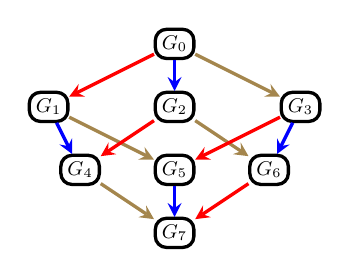
\begin{tikzpicture}[
    scale=0.8,
    transform shape,
    >=stealth,
    node distance=2.2cm and 2.5cm,
    hypernode/.style={draw, rectangle, rounded corners=4pt, very thick, inner sep=3pt, font=\small\bfseries},
    edge label/.style={midway, very thick,
    fill=white, font=\footnotesize, inner sep=1pt},
    edge-t1/.style={->, very thick, Red},
    edge-t2/.style={->, very thick, blue},
    edge-t3/.style={->, very thick, Dandelion!60!black}
]

% Top layer: G0
\node[hypernode] (G0) at (0,0) {$G_0$};

% Second layer
\node[hypernode] (G1) at (-2,-1) {$G_1$};
\node[hypernode] (G2) at (0,-1) {$G_2$};
\node[hypernode] (G3) at (2,-1) {$G_3$};

% Third layer
\node[hypernode] (G4) at (-1.5,-2) {$G_4$};
\node[hypernode] (G5) at (0,-2) {$G_5$};
\node[hypernode] (G6) at (1.5,-2) {$G_6$};

% Last layer
\node[hypernode] (G7) at (0,-3) {$G_7$};

% Edges from G0
\draw[edge-t1] (G0) -- (G1);
\draw[edge-t2] (G0) -- (G2);
\draw[edge-t3] (G0) -- (G3);

% Edges from G1
\draw[edge-t2] (G1) -- (G4);
\draw[edge-t3] (G1) -- (G5);

% Edges from G2
\draw[edge-t1] (G2) -- (G4);
\draw[edge-t3] (G2) -- (G6);

% Edges from G3
\draw[edge-t1] (G3) -- (G5);
\draw[edge-t2] (G3) -- (G6);

% Edges to G7
\draw[edge-t3] (G4) -- (G7);
\draw[edge-t2] (G5) -- (G7);
\draw[edge-t1] (G6) -- (G7);

\end{tikzpicture}
\label{hypergraph-rrr}


% \begin{figure}[t]
% \centering
% \resizebox{0.5\textwidth}{!}{ 
% \begin{tikzpicture}[
%     >=stealth,
%     node distance=1.4cm and 1.8cm,
%     event/.style={draw=none, font=\normalsize},
%     rf/.style={->, thick, dashed, green!60!black},
%     co/.style={->, thick, dotted, red!80!black},
%     hyper edge/.style={->, thick, blue!70!black},
%     graph box/.style={draw, rectangle, rounded corners=4pt, thick, minimum width=1.4cm, minimum height=1cm, inner sep=0.1cm, minimum size=0cm},
%     scale=0.65,
%     every node/.style={transform shape}
% ]

% % First row: G0, G1, G2, G3
% % G0
% \begin{scope}[xshift=-2cm, yshift=0cm, local bounding box=G0box]
%   \node[event] (g0i) {$\init$};
% \end{scope}
% \node[graph box, fit=(G0box)] (G0) {};

% % G1
% \begin{scope}[xshift=-6cm, yshift=-2cm, local bounding box=G1box]
%   \node[event] (g1i) {$\init$};
%   \node[event, below=0.7cm of g1i, xshift=-1.0cm] (g1r1) {$$\opr(x)$$};
%   \draw[->] (g1i) -- node[midway, left, font=\small] {$t_1$} (g1r1);
% \end{scope}
% \node[graph box, fit=(G1box)] (G1) {};

% % G2
% \begin{scope}[xshift=-2cm, yshift=-2cm, local bounding box=G2box]
%   \node[event] (g2i) {$\init$};
%   \node[event, below=0.7cm of g2i] (g2r2) {$$\opr(x)$$};
%   \draw[->] (g2i) -- node[midway, right, font=\small] {$t_2$}(g2r2);
% \end{scope}
% \node[graph box, fit=(G2box)] (G2) {};

% % G3
% \begin{scope}[xshift=2cm, yshift=-2cm, local bounding box=G3box]
%   \node[event] (g3i) {$\init$};
%   \node[event, below=0.7cm of g3i, xshift=1.0cm] (g3r3) {$$\opr(x)$$};
%   \draw[->] (g3i) -- node[midway, right, xshift=0.3cm, font=\small] {$t_3$}(g3r3);
% \end{scope}
% \node[graph box, fit=(G3box)] (G3) {};

% % Second row: G4, G5, G6
% % G4
% \begin{scope}[xshift=-6cm, yshift=-6cm, local bounding box=G4box]
%   \node[event] (g4i) {$\init$};
%   \node[event, below=0.7cm of g4i, xshift=-1.0cm] (g4r1) {$$\opr(x)$$};
%   \node[event, below=0.7cm of g4i] (g4r2) {$$\opr(x)$$};
%   \draw[->] (g4i) -- node[midway, left, font=\small] {$t_1$}(g4r1);
%   \draw[->] (g4i) -- node[midway, right, font=\small] {$t_2$}(g4r2);
% \end{scope}
% \node[graph box, fit=(G4box)] (G4) {};

% % G5
% \begin{scope}[xshift=-2cm, yshift=-6cm, local bounding box=G5box]
%   \node[event] (g5i) {$\init$};
%   \node[event, below=0.7cm of g5i, xshift=-1.0cm] (g5r1) {$$\opr(x)$$};
%   \node[event, below=0.7cm of g5i, xshift=1.0cm] (g5r3) {$$\opr(x)$$};
%   \draw[->] (g5i) -- node[midway, left, font=\small] {$t_1$}(g5r1);
%   \draw[->] (g5i) -- node[midway, right, xshift=0.3cm, font=\small] {$t_3$}(g5r3);
% \end{scope}
% \node[graph box, fit=(G5box)] (G5) {};

% % G6
% \begin{scope}[xshift=2cm, yshift=-6cm, local bounding box=G6box]
%   \node[event] (g6i) {$\init$};
%   \node[event, below=0.7cm of g6i] (g6r2) {$$\opr(x)$$};
%   \node[event, below=0.7cm of g6i, xshift=1.0cm] (g6r3) {$$\opr(x)$$};
%   \draw[->] (g6i) -- node[midway, right, font=\small] {$t_2$}(g6r2);
%   \draw[->] (g6i) -- node[midway, right, xshift=0.3cm, font=\small] {$t_3$}(g6r3);
% \end{scope}
% \node[graph box, fit=(G6box)] (G6) {};

% % Third row: G7
% % G7
% \begin{scope}[xshift=-2cm, yshift=-10cm, local bounding box=G7box]
%   \node[event] (g7i) {$\init$};
%   \node[event, below=0.7cm of g7i, xshift=-1.2cm] (g7r1) {$$\opr(x)$$};
%   \node[event, below=0.7cm of g7i] (g7r2) {$$\opr(x)$$};
%   \node[event, below=0.7cm of g7i, xshift=1.2cm] (g7r3) {$$\opr(x)$$};
%   \draw[->] (g7i) -- node[midway, left, font=\small] {$t_1$}(g7r1);
%   \draw[->] (g7i) -- node[midway, right, font=\small] {$t_2$}(g7r2);
%   \draw[->] (g7i) -- node[midway, right, xshift=0.3cm, font=\small] {$t_3$}(g7r3);
% \end{scope}
% \node[graph box, fit=(G7box)] (G7) {};

% % Hyperedges - First layer
% \draw[hyper edge] (G0) -- node[midway, above left, font=\small] {$t_1$} (G1);
% \draw[hyper edge] (G0) -- node[midway, above, font=\small] {$t_2$} (G2);
% \draw[hyper edge] (G0) -- node[midway, above right, font=\small] {$t_3$} (G3);

% % Hyperedges - Second layer
% \draw[hyper edge] (G1) -- node[midway, above left, font=\small] {$t_2$} (G4);
% \draw[hyper edge] (G1) -- node[midway, above right, font=\small] {$t_3$} (G5);
% \draw[hyper edge] (G2) -- node[midway, above left, font=\small] {$t_1$} (G4);
% \draw[hyper edge] (G2) -- node[midway, above right, font=\small] {$t_3$} (G6);
% \draw[hyper edge] (G3) -- node[midway, above left, font=\small] {$t_1$} (G5);
% \draw[hyper edge] (G3) -- node[midway, above right, font=\small] {$t_2$} (G6);

% % Hyperedges - Third layer
% \draw[hyper edge] (G4) -- node[midway, above left, font=\small] {$t_3$} (G7);
% \draw[hyper edge] (G5) -- node[midway, above, font=\small] {$t_2$} (G7);
% \draw[hyper edge] (G6) -- node[midway, above right, font=\small] {$t_1$} (G7);
% \end{tikzpicture}
% }
% \caption{The meta-graph of the \cref{ex:r+r+r}}
% \label{fig:rrr}
% \end{figure}

%%%%%%%%%%%% Hyper Node Graphs
% \begin{figure}
% \centering
% \begin{tikzpicture}[
%     >=stealth,
%     node distance=1.4cm and 1.8cm,
%     event/.style={draw=none, font=\small},
%     rf/.style={->, thick, dashed, green!60!black},
%     co/.style={->, thick, dotted, red!80!black},
%     ->, thick
% ]

% % First row:

% %G0
% \begin{scope}[xshift=0cm, yshift=0cm]
%   \node[event] (g0i) {$\init$};
%   \node[below=1.2cm of g0i] {(G0)};
% \end{scope}

% %G1
% \begin{scope}[xshift=3cm, yshift=0cm]
%   \node[event] (g1i) {$\init$};
%   \node[event, below=0.7cm of g1i, xshift=-1.2cm] (g1r1) {$$\opr(x)$$};
%   \draw[->] (g1i) -- node[midway, left] {$t_1$} (g1r1);
%   \node[below=1.2cm of g1i] {(G1)};
% \end{scope}

% %G2
% \begin{scope}[xshift=6cm, yshift=0cm]
%   \node[event] (g2i) {$\init$};
%   \node[event, below=0.7cm of g2i] (g2r2) {$$\opr(x)$$};
%   \draw[->] (g2i) -- node[midway, right] {$t_2$}(g2r2);
%   \node[below=1.2cm of g2i] {(G2)};
% \end{scope}

% %G3
% \begin{scope}[xshift=9cm, yshift=0cm]
%   \node[event] (g3i) {$\init$};
%    \node[event, below=0.7cm of g3i, xshift=1.2cm] (g3r3) {$$\opr(x)$$};
%   \draw[->] (g3i) -- node[midway, right, xshift=0.3cm] {$t_3$}(g3r3);
%   \node[below=1.2cm of g3i] {(G3)};
% \end{scope}

% %Second Row:

% %G4
% \begin{scope}[xshift=0cm, yshift=-2.5cm]
%   \node[event] (g4i) {$\init$};
%   \node[event, below=0.7cm of g4i, xshift=-1.2cm] (g4r1) {$$\opr(x)$$};
%   \node[event, below=0.7cm of g4i] (g4r2) {$$\opr(x)$$};
%   \draw[->] (g4i) -- node[midway, left] {$t_1$}(g4r1);
%   \draw[->] (g4i) -- node[midway, right] {$t_2$}(g4r2);
%   \node[below=1.2cm of g4i] {(G4)};
% \end{scope}

% % %G5
% \begin{scope}[xshift=3cm, yshift=-2.5cm]
%   \node[event] (g5i) {$\init$};
%   \node[event, below=0.7cm of g5i, xshift=-1.2cm] (g5r1) {$$\opr(x)$$};
%   \node[event, below=0.7cm of g5i, xshift=1.2cm] (g5r3) {$$\opr(x)$$};
%   \draw[->] (g5i) -- node[midway, left] {$t_1$}(g5r1);
%   \draw[->] (g5i) -- node[midway, right, xshift=0.3cm] {$t_3$}(g5r3);
%   \node[below=1.2cm of g5i] {(G5)};
% \end{scope}

% %G6
% \begin{scope}[xshift=6cm, yshift=-2.5cm]
%   \node[event] (g6i) {$\init$};
%   \node[event, below=0.7cm of g6i] (g7r2) {$$\opr(x)$$};
%   \node[event, below=0.7cm of g6i, xshift=1.2cm] (g7r3) {$$\opr(x)$$};
%   \draw[->] (g6i) -- node[midway, right] {$t_2$}(g7r2);
%   \draw[->] (g6i) -- node[midway, right, xshift=0.3cm] {$t_3$}(g7r3);
%   \node[below=1.2cm of g6i] {(G6)};
% \end{scope}

% %G7
% \begin{scope}[xshift=9cm, yshift=-2.5cm]
%   \node[event] (g7i) {$\init$};
%   \node[event, below=0.7cm of g7i, xshift=-1.2cm] (g7r1) {$$\opr(x)$$};
%   \node[event, below=0.7cm of g7i] (g7r2) {$$\opr(x)$$};
%   \node[event, below=0.7cm of g7i, xshift=1.2cm] (g7r3) {$$\opr(x)$$};
%   \draw[->] (g7i) -- node[midway, left] {$t_1$}(g7r1);
%   \draw[->] (g7i) -- node[midway, right] {$t_2$}(g7r2);
%   \draw[->] (g7i) -- node[midway, right, xshift=0.3cm] {$t_3$}(g7r3);
%   \node[below=1.2cm of g7i] {(G7)};
% \end{scope}
% \end{tikzpicture}
% \caption{The meta-graph of the RRR example}
% \label{meta-graph-rrr}
% \end{figure}

% %%%%%%%%%%% Abstract Hyper-graph
% \begin{figure}
% \centering
% \begin{tikzpicture}[
%     >=stealth,
%     node distance=2.2cm and 2.5cm,
%     hypernode/.style={draw, rectangle, rounded corners=4pt, thick, minimum width=1.4cm, minimum height=1cm, font=\small\bfseries},
%     edge label/.style={midway, fill=white, font=\footnotesize, inner sep=1pt}
% ]

% % Top layer: G0
% \node[hypernode] (G0) at (0,0) {G0};

% % Second layer
% \node[hypernode] (G1) at (-3,-2) {G1};
% \node[hypernode] (G2) at (0,-2) {G2};
% \node[hypernode] (G3) at (3,-2) {G3};

% % Third layer
% \node[hypernode] (G4) at (-2.5,-4.2) {G4};
% \node[hypernode] (G5) at (0,-4.2) {G5};
% \node[hypernode] (G6) at (2.5,-4.2) {G6};

% % Last layer
% \node[hypernode] (G7) at (0,-6.4) {G7};

% % Edges from G0
% \draw[->] (G0) -- (G1);
% \draw[->] (G0) -- (G2);
% \draw[->] (G0) -- (G3) ;

% % Edges from G1
% \draw[->] (G1) -- (G4);
% \draw[->] (G1) -- (G5);

% % Edges from G2
% \draw[->] (G2) -- (G4);
% \draw[->] (G2) -- (G6);

% % Edges from G3
% \draw[->] (G3) -- (G5);
% \draw[->] (G3) -- (G6);

% % Edges to G7
% \draw[->] (G4) -- (G7) ;
% \draw[->] (G5) -- (G7) ;
% \draw[->] (G6) -- (G7) ;

% \end{tikzpicture}
% \caption{Abstract hypergraph for the RRR example}
% \label{hypergraph-rrr}
% \end{figure}

\end{minipage}%
\end{tcolorbox}


\subsection{Pitt Estimation}

The above disadvantage of \textbf{Algorithm K} on DAGs can be rectified:
Pitt \cite{pitt} showed that \textbf{Algorithm K} can be adapted to estimate the number of sinks in a DAG. 
The key idea is to correct for overcounting at each step,  by dividing  the multiplicative weight with the  number of incoming edges to the current node.

\begin{verse}
\textbf{Algorithm P} \cite{pitt}.
Given a DAG $T$, run the following randomized procedure.
Starting at the root, for each node $n_i$ with $d_i$ children and $e_i$ incoming edges,
pick a child uniformly at random and move there, until reaching a node $n_k$ with no outgoing edges.
Stop and output $\frac{d_1}{e_1} \ldots \frac{d_k}{e_k}$.
In the algorithm, we assume $e_1 = 1$ for the root and $d_k = 1$ for the leaf.
\end{verse}


\begin{proposition}
For any program $P$, \textbf{Algorithm P} is a poly-time unbiased estimator for $C(P)$.
\end{proposition}

\begin{tcolorbox}[
    colback=SkyBlue!5,
    colframe=blue!20,
    boxrule=1pt,
    arc=2pt,
    width=\textwidth,
    breakable
]
\begin{example}
For \cref{ex:r+r+r}, \textbf{Algorithm P} estimates $(3\times 2\times 1 \times 1)/(1\times 1 \times 2\times 3) = 1$ for each path through the DAG.
Thus, the expectation is also 1 (and the variance is 0).
\qed
\end{example}
\end{tcolorbox}
To show that \textbf{Algorithm P} is poly-time, given an execution graph, we have to determine the number of its \emph{incoming} edges in $\mathcal{T}(P)$ in poly-time.
For sequentially consistent executions, we can do this as follows.
Let $G=(E,\rf{},\mo{})$ be an execution graph.
An event $e\in G.E$ is said to be sequentially maximal if it is maximal with respect to the $\seqcon{}$ relation. 
%An event $e\in G.E$ is said to be sequentially maximal, written \emph{$\seqcon{}^{\max}(e)$}, if it is maximal with respect to the $\seqcon{}$ relation. 
%We define the set of all $\seqcon{}^{\max}$ events of $G$ as $\seqcon{}^{\max}(G) = \{e \mid \forall e' \in G.E : (e,e') \not\in G.\seqcon{}\}$.

\begin{proposition}
\label{prop1}
Let $P$ be a program and let $G$ a reachable execution graph in $\mathcal{T}(P)$. 
The number of predecessors of $G$ is exactly the number of sequentially maximal events of $G$. 
\end{proposition}

The proof can be found in \cref{theory:C}.
Since it is easily seen that we can compute the number of sequentially maximal events of an execution graph in polynomial-time,
Proposition~\ref{prop1} implies that \textbf{Algorithm P} is poly-time.

%Proposition~\ref{prop1} implies that the number of predecessors of each node in the DAG $\mathcal{T}(P)$ 
%can be computed by computing $\seqcon{}^{\max}$ which can be done in polynomial time. Thus, \textbf{Algorithm P} is poly-time.

\begin{comment}
\begin{example}
Unfortunately, Algorithm P can have very high variance.
Consider the program
\begin{equation*}
  \tag{\textsc{rlru+rlru}}
  \label{ex:rlru+rlru}
  \inarr{ 
\readInst{a_1}{x} \\
\lockInst{l}\\
\readInst{b_1}{y}\\
\unlockInst{l}
}{ 
\readInst{a_2}{x} \\
\lockInst{l}\\
\readInst{b_2}{y}\\
\unlockInst{l}
}
\end{equation*}
It has exactly two execution graphs, depending on whether the first or the second thread wins the race on the lock.
However, 
\RM{Mohammad fill in the rest}
\qed
\end{example}

\begin{figure}[htbp]
\centering
\resizebox{0.6\textwidth}{!}{ 
\begin{tikzpicture}[
    >=stealth,
    node distance=1.4cm and 1.8cm,
    event/.style={draw=none, font=\normalsize},
    rf/.style={->, thick, dashed, green!60!black},
    co/.style={->, very thick, dotted, red!80!black},
    hyper edge/.style={->, thick, blue!70!black},
    graph box/.style={draw, rectangle, rounded corners=4pt, thick, minimum width=1.4cm, minimum height=1cm, inner sep=0.1cm, minimum size=0cm},
    scale=0.65,
    every node/.style={transform shape}
]

% First row: G0, G1, G2, G3
% G0
\begin{scope}[xshift=0cm, yshift=0cm, local bounding box=G0box]
  \node[event] (g0i) {$\init$};
\end{scope}
\node[graph box, fit=(G0box)] (G0) {};

% G1
\begin{scope}[xshift=-4cm, yshift=-2cm, local bounding box=G1box]
  \node[event] (g1i) {$\init$};
  \node[event, below=0.7cm of g1i, xshift=-1.0cm] (g1r1) {$\opr(x)$};
  \draw[->] (g1i) -- (g1r1);
\end{scope}
\node[graph box, fit=(G1box)] (G1) {};

% G2
\begin{scope}[xshift=4cm, yshift=-2cm, local bounding box=G2box]
  \node[event] (g2i) {$\init$};
  \node[event, below=0.7cm of g2i, xshift=1.0cm]  (g2r2) {$\opr(x)$};
  \draw[->] (g2i) -- (g2r2);
\end{scope}
\node[graph box, fit=(G2box)] (G2) {};


% G3
\begin{scope}[xshift=-7cm, yshift=-5cm, local bounding box=G3box]
  \node[event] (g3i) {$\init$};
  \node[event, below=0.7cm of g3i, xshift=-1.0cm] (g3r1) {$\opr(x)$};
  \node[event, below=0.4cm of g3r1] (g3l2) {$\opaq(l)$};
  \draw[->] (g3i) -- (g3r1);
  \draw[->] (g3r1) -- (g3l2);
  \draw[rf] (g3i) to[bend left=15] (g3l2);
\end{scope}
\node[graph box, fit=(G3box)] (G3) {};

% G4
\begin{scope}[xshift=0cm, yshift=-5cm, local bounding box=G4box]
  \node[event] (g4i) {$\init$};
  \node[event, below=0.7cm of g4i, xshift=-1.0cm] (g4r1) {$\opr(x)$};
  \node[event, below=0.7cm of g4i, xshift=1.0cm]  (g4r2) {$\opr(x)$};
  \draw[->] (g4i) -- (g4r1);
  \draw[->] (g4i) -- (g4r2);
\end{scope}
\node[graph box, fit=(G4box)] (G4) {};

% G5
\begin{scope}[xshift=7cm, yshift=-5cm, local bounding box=G5box]
  \node[event] (g5i) {$\init$};
  \node[event, below=0.7cm of g5i, xshift=1.0cm] (g5r1) {$\opr(x)$};
  \node[event, below=0.4cm of g5r1] (g5l2) {$\opaq(l)$};
  \draw[->] (g5i) -- (g5r1);
  \draw[->] (g5r1) -- (g5l2);
  \draw[rf] (g5i) to[bend right=15] (g5l2);
\end{scope}
\node[graph box, fit=(G5box)] (G5) {};

% G6
\begin{scope}[xshift=-10cm, yshift=-8cm, local bounding box=G6box]
  \node[event] (g6i) {$\init$};
  \node[event, below=0.7cm of g6i, xshift=-1.0cm] (g6r1) {$\opr(x)$};
  \node[event, below=0.4cm of g6r1] (g6l2) {$\opaq(l)$};
  \node[event, below=0.4cm of g6l2] (g6r3) {$\opr(y)$};
  \draw[->] (g6i) -- (g6r1);
  \draw[->] (g6r1) -- (g6l2);
  \draw[->] (g6l2) -- (g6r3);
  \draw[rf] (g6i) to[bend left=15] (g6l2);
\end{scope}
\node[graph box, fit=(G6box)] (G6) {};

% G7
\begin{scope}[xshift=-4cm, yshift=-8cm, local bounding box=G7box]
  \node[event] (g7i) {$\init$};
  \node[event, below=0.7cm of g7i, xshift=-1.0cm] (g7r1) {$\opr(x)$};
  \node[event, below=0.4cm of g7r1] (g7l2) {$\opaq(l)$};
  \node[event, below=0.7cm of g7i, xshift=1.0cm]  (g7r3) {$\opr(x)$};
  \draw[->] (g7i) -- (g7r1);
  \draw[->] (g7r1) -- (g7l2);
  \draw[->] (g7i) -- (g7r3);
  \draw[rf] (g7i) to[bend left=15] (g7l2);
\end{scope}
\node[graph box, fit=(G7box)] (G7) {};

% G8
\begin{scope}[xshift=4cm, yshift=-8cm, local bounding box=G8box]
  \node[event] (g8i) {$\init$};
  \node[event, below=0.7cm of g8i, xshift=-1.0cm] (g8r1) {$\opr(x)$};
  \node[event, below=0.7cm of g8i, xshift=1.0cm] (g8r2) {$\opr(x)$};
  \node[event, below=0.4cm of g8r2] (g8l3) {$\opaq(l)$};
  \draw[->] (g8i) -- (g8r1);
  \draw[->] (g8i) -- (g8r2);
  \draw[->] (g8r2) -- (g8l3);
  \draw[rf] (g8i) to[bend right=15] (g8l3);
\end{scope}
\node[graph box, fit=(G8box)] (G8) {};

% G9
\begin{scope}[xshift=10cm, yshift=-8cm, local bounding box=G9box]
  \node[event] (g9i) {$\init$};
  \node[event, below=0.7cm of g9i, xshift=1.0cm] (g9r1) {$\opr(x)$};
  \node[event, below=0.4cm of g9r1] (g9l2) {$\opaq(l)$};
  \node[event, below=0.4cm of g9l2] (g9r3) {$\opr(y)$};
  \draw[->] (g9i) -- (g9r1);
  \draw[->] (g9r1) -- (g9l2);
  \draw[->] (g9l2) -- (g9r3);
  \draw[rf] (g9i) to[bend right=15] (g9l2);
\end{scope}
\node[graph box, fit=(G9box)] (G9) {};

% G10
\begin{scope}[xshift=-10cm, yshift=-13cm, local bounding box=G10box]
  \node[event] (g10i) {$\init$};
  \node[event, below=0.7cm of g10i, xshift=-1.0cm] (g10r1) {$\opr(x)$};
  \node[event, below=0.4cm of g10r1] (g10l2) {$\opaq(l)$};
  \node[event, below=0.4cm of g10l2] (g10r3) {$\opr(y)$};
  \node[event, below=0.4cm of g10r3] (g10l4) {$\oprl(l)$};
  \draw[->] (g10i) -- (g10r1);
  \draw[->] (g10r1) -- (g10l2);
  \draw[->] (g10l2) -- (g10r3);
  \draw[->] (g10r3) -- (g10l4);
  \draw[rf] (g10i) to[bend left=15] (g10l2);
\end{scope}
\node[graph box, fit=(G10box)] (G10) {};

% G11
\begin{scope}[xshift=-4cm, yshift=-13cm, local bounding box=G11box]
  \node[event] (g11i) {$\init$};
  \node[event, below=0.7cm of g11i, xshift=-1.0cm] (g11r1) {$\opr(x)$};
  \node[event, below=0.4cm of g11r1] (g11l2) {$\opaq(l)$};
  \node[event, below=0.7cm of g11i, xshift=1.0cm]  (g11r3) {$\opr(x)$};
  \node[event, below=0.4cm of g11l2] (g11r4) {$\opr(y)$};
  \draw[->] (g11i) -- (g11r1);
  \draw[->] (g11r1) -- (g11l2);
  \draw[->] (g11l2) -- (g11r4);
  \draw[->] (g11i) -- (g11r3);
  \draw[rf] (g11i) to[bend left=15] (g11l2);
\end{scope}
\node[graph box, fit=(G11box)] (G11) {};

% G12
\begin{scope}[xshift=4cm, yshift=-13cm, local bounding box=G12box]
  \node[event] (g12i) {$\init$};
  \node[event, below=0.7cm of g12i, xshift=-1.0cm] (g12r1) {$\opr(x)$};
  \node[event, below=0.7cm of g12i, xshift=1.0cm] (g12r2) {$\opr(x)$};
  \node[event, below=0.4cm of g12r2] (g12l3) {$\opaq(l)$};
  \node[event, below=0.4cm of g12l3] (g12r4) {$\opr(y)$};
  \draw[->] (g12i) -- (g12r1);
  \draw[->] (g12i) -- (g12r2);
  \draw[->] (g12r2) -- (g12l3);
  \draw[->] (g12l3) -- (g12r4);
  \draw[rf] (g12i) to[bend right=15] (g12l3);
\end{scope}
\node[graph box, fit=(G12box)] (G12) {};

% G13
\begin{scope}[xshift=10cm, yshift=-13cm, local bounding box=G13box]
  \node[event] (g13i) {$\init$};
  \node[event, below=0.7cm of g13i, xshift=1.0cm] (g13r1) {$\opr(x)$};
  \node[event, below=0.4cm of g13r1] (g13l2) {$\opaq(l)$};
  \node[event, below=0.4cm of g13l2] (g13r3) {$\opr(y)$};
  \node[event, below=0.4cm of g13r3] (g13l4) {$\oprl(l)$};
  \draw[->] (g13i) -- (g13r1);
  \draw[->] (g13r1) -- (g13l2);
  \draw[->] (g13l2) -- (g13r3);
  \draw[->] (g13r3) -- (g13l4);
  \draw[rf] (g13i) to[bend right=15] (g13l2);
\end{scope}
\node[graph box, fit=(G13box)] (G13) {};

% G14
\begin{scope}[xshift=-7cm, yshift=-18cm, local bounding box=G14box]
  \node[event] (g14i) {$\init$};
  \node[event, below=0.7cm of g14i, xshift=-1.0cm] (g14r1) {$\opr(x)$};
  \node[event, below=0.4cm of g14r1] (g14l2) {$\opaq(l)$};
  \node[event, below=0.7cm of g14i, xshift=1.0cm]  (g14r3) {$\opr(x)$};
  \node[event, below=0.4cm of g14l2] (g14r4) {$\opr(y)$};
  \node[event, below=0.4cm of g14r4] (g14l5) {$\oprl(l)$};
  \draw[->] (g14i) -- (g14r1);
  \draw[->] (g14r1) -- (g14l2);
  \draw[->] (g14l2) -- (g14r4);
  \draw[->] (g14r4) -- (g14l5);
  \draw[->] (g14i) -- (g14r3);
  \draw[rf] (g14i) to[bend left=15] (g14l2);
\end{scope}
\node[graph box, fit=(G14box)] (G14) {};

% G15
\begin{scope}[xshift=7cm, yshift=-18cm, local bounding box=G15box]
  \node[event] (g15i) {$\init$};
  \node[event, below=0.7cm of g15i, xshift=-1.0cm] (g15r1) {$\opr(x)$};
  \node[event, below=0.7cm of g15i, xshift=1.0cm] (g15r2) {$\opr(x)$};
  \node[event, below=0.4cm of g15r2] (g15l3) {$\opaq(l)$};
  \node[event, below=0.4cm of g15l3] (g15r4) {$\opr(y)$};
  \node[event, below=0.4cm of g15r4] (g15l5) {$\oprl(l)$};
  \draw[->] (g15i) -- (g15r1);
  \draw[->] (g15i) -- (g15r2);
  \draw[->] (g15r2) -- (g15l3);
  \draw[->] (g15l3) -- (g15r4);
  \draw[->] (g15r4) -- (g15l5);
  \draw[rf] (g15i) to[bend right=15] (g15l3);
\end{scope}
\node[graph box, fit=(G15box)] (G15) {};

% G16
\begin{scope}[xshift=-7cm, yshift=-24cm, local bounding box=G16box]
  \node[event] (g16i) {$\init$};
  \node[event, below=0.7cm of g16i, xshift=-1.0cm] (g16r1) {$\opr(x)$};
  \node[event, below=0.4cm of g16r1] (g16l2) {$\opaq(l)$};
  \node[event, below=0.7cm of g16i, xshift=1.0cm]  (g16r3) {$\opr(x)$};
  \node[event, below=0.4cm of g16l2] (g16r4) {$\opr(y)$};
  \node[event, below=0.4cm of g16r4] (g16l5) {$\oprl(l)$};
    \node[event, below=0.4cm of g16r3] (g16l6) {$\opaq(l)$};
  \draw[->] (g16i) -- (g16r1);
  \draw[->] (g16r1) -- (g16l2);
  \draw[->] (g16l2) -- (g16r4);
  \draw[->] (g16r4) -- (g16l5);
  \draw[->] (g16i) -- (g16r3);
  \draw[->] (g16r3) -- (g16l6);
  \draw[rf] (g16i) to[bend left=15] (g16l2);
  \draw[rf] (g16l5) to[] (g16l6);
\end{scope}
\node[graph box, fit=(G16box)] (G16) {};

% G17
\begin{scope}[xshift=7cm, yshift=-24cm, local bounding box=G17box]
  \node[event] (g17i) {$\init$};
  \node[event, below=0.7cm of g17i, xshift=-1.0cm] (g17r1) {$\opr(x)$};
  \node[event, below=0.7cm of g17i, xshift=1.0cm] (g17r2) {$\opr(x)$};
  \node[event, below=0.4cm of g17r2] (g17l3) {$\opaq(l)$};
  \node[event, below=0.4cm of g17l3] (g17r4) {$\opr(y)$};
  \node[event, below=0.4cm of g17r4] (g17l5) {$\oprl(l)$};
  \node[event, below=0.4cm of g17r1] (g17l6) {$\opaq(l)$};
  \draw[->] (g17i) -- (g17r1);
  \draw[->] (g17r1) -- (g17l6);
  \draw[->] (g17i) -- (g17r2);
  \draw[->] (g17r2) -- (g17l3);
  \draw[->] (g17l3) -- (g17r4);
  \draw[->] (g17r4) -- (g17l5);
  \draw[rf] (g17i) to[bend right=15] (g17l3);
  \draw[rf] (g17l5) to[] (g17l6);
\end{scope}
\node[graph box, fit=(G17box)] (G17) {};

% G18
\begin{scope}[xshift=-7cm, yshift=-30cm, local bounding box=G18box]
  \node[event] (g18i) {$\init$};
  \node[event, below=0.7cm of g18i, xshift=-1.0cm] (g18r1) {$\opr(x)$};
  \node[event, below=0.4cm of g18r1] (g18l2) {$\opaq(l)$};
  \node[event, below=0.7cm of g18i, xshift=1.0cm]  (g18r3) {$\opr(x)$};
  \node[event, below=0.4cm of g18l2] (g18r4) {$\opr(y)$};
  \node[event, below=0.4cm of g18r4] (g18l5) {$\oprl(l)$};
    \node[event, below=0.4cm of g18r3] (g18l6) {$\opaq(l)$};
    \node[event, below=0.4cm of g18l6] (g18r7) {$\opr(y)$};
  \draw[->] (g18i) -- (g18r1);
  \draw[->] (g18r1) -- (g18l2);
  \draw[->] (g18l2) -- (g18r4);
  \draw[->] (g18r4) -- (g18l5);
  \draw[->] (g18i) -- (g18r3);
  \draw[->] (g18r3) -- (g18l6);
  \draw[->] (g18l6) -- (g18r7);
  \draw[rf] (g18i) to[bend left=15] (g18l2);
  \draw[rf] (g18l5) to[] (g18l6);
\end{scope}
\node[graph box, fit=(G18box)] (G18) {};

% G19
\begin{scope}[xshift=7cm, yshift=-30cm, local bounding box=G19box]
  \node[event] (g19i) {$\init$};
  \node[event, below=0.7cm of g19i, xshift=-1.0cm] (g19r1) {$\opr(x)$};
  \node[event, below=0.7cm of g19i, xshift=1.0cm] (g19r2) {$\opr(x)$};
  \node[event, below=0.4cm of g19r2] (g19l3) {$\opaq(l)$};
  \node[event, below=0.4cm of g19l3] (g19r4) {$\opr(y)$};
  \node[event, below=0.4cm of g19r4] (g19l5) {$\oprl(l)$};
  \node[event, below=0.4cm of g19r1] (g19l6) {$\opaq(l)$};
  \node[event, below=0.4cm of g19l6] (g19r7) {$\opr(y)$};
  \draw[->] (g19i) -- (g19r1);
  \draw[->] (g19r1) -- (g19l6);
  \draw[->] (g19l6) -- (g19r7);
  \draw[->] (g19i) -- (g19r2);
  \draw[->] (g19r2) -- (g19l3);
  \draw[->] (g19l3) -- (g19r4);
  \draw[->] (g19r4) -- (g19l5);
  \draw[rf] (g19i) to[bend right=15] (g19l3);
  \draw[rf] (g19l5) to[] (g19l6);
\end{scope}
\node[graph box, fit=(G19box)] (G19) {};

% G20
\begin{scope}[xshift=-7cm, yshift=-36cm, local bounding box=G20box]
  \node[event] (g20i) {$\ini$};
  \node[event, below=0.7cm of g20i, xshift=-1.0cm] (g20r1) {$\opr(x)$};
  \node[event, below=0.4cm of g20r1] (g20l2) {$\opaq(l)$};
  \node[event, below=0.7cm of g20i, xshift=1.0cm]  (g20r3) {$\opr(x)$};
  \node[event, below=0.4cm of g20l2] (g20r4) {$\opr(y)$};
  \node[event, below=0.4cm of g20r4] (g20l5) {$\oprl(l)$};
    \node[event, below=0.4cm of g20r3] (g20l6) {$\opaq(l)$};
    \node[event, below=0.4cm of g20l6] (g20r7) {$\opr(y)$};
    \node[event, below=0.4cm of g20r7] (g20l8) {$\oprl(l)$};
  \draw[->] (g20i) -- (g20r1);
  \draw[->] (g20r1) -- (g20l2);
  \draw[->] (g20l2) -- (g20r4);
  \draw[->] (g20r4) -- (g20l5);
  \draw[->] (g20i) -- (g20r3);
  \draw[->] (g20r3) -- (g20l6);
  \draw[->] (g20l6) -- (g20r7);
  \draw[->] (g20r7) -- (g20l8);
  \draw[rf] (g20i) to[bend left=15] (g20l2);
  \draw[rf] (g20l5) to[] (g20l6);
\end{scope}
\node[graph box, fit=(G20box)] (G20) {};

% G21
\begin{scope}[xshift=7cm, yshift=-36cm, local bounding box=G21box]
  \node[event] (g21i) {$\init$};
  \node[event, below=0.7cm of g21i, xshift=-1.0cm] (g21r1) {$\opr(x)$};
  \node[event, below=0.7cm of g21i, xshift=1.0cm] (g21r2) {$\opr(x)$};
  \node[event, below=0.4cm of g21r2] (g21l3) {$\opaq(l)$};
  \node[event, below=0.4cm of g21l3] (g21r4) {$\opr(y)$};
  \node[event, below=0.4cm of g21r4] (g21l5) {$\oprl(l)$};
  \node[event, below=0.4cm of g21r1] (g21l6) {$\opaq(l)$};
  \node[event, below=0.4cm of g21l6] (g21r7) {$\opr(y)$};
  \node[event, below=0.4cm of g21r7] (g21l8) {$\oprl(l)$};
  \draw[->] (g21i) -- (g21r1);
  \draw[->] (g21r1) -- (g21l6);
  \draw[->] (g21l6) -- (g21r7);
  \draw[->] (g21r7) -- (g21l8);
  \draw[->] (g21i) -- (g21r2);
  \draw[->] (g21r2) -- (g21l3);
  \draw[->] (g21l3) -- (g21r4);
  \draw[->] (g21r4) -- (g21l5);
  \draw[rf] (g21i) to[bend right=15] (g21l3);
  \draw[rf] (g21l5) to[] (g21l6);
\end{scope}
\node[graph box, fit=(G21box)] (G21) {};

% Hyperedges - First layer
\draw[hyper edge] (G0) -- node[midway, above left, font=\small] {$t_1$} (G1);
\draw[hyper edge] (G0) -- node[midway, above, font=\small] {$t_2$} (G2);
\draw[hyper edge] (G1) -- node[midway, above, font=\small] {$t_1$} (G3);
\draw[hyper edge] (G1) -- node[midway, above, font=\small] {$t_2$} (G4);
\draw[hyper edge] (G2) -- node[midway, above, font=\small] {$t_1$} (G4);
\draw[hyper edge] (G2) -- node[midway, above, font=\small] {$t_2$} (G5);
\draw[hyper edge] (G3) -- node[midway, above, font=\small] {$t_1$} (G6);
\draw[hyper edge] (G3) -- node[midway, above, font=\small] {$t_2$} (G7);
\draw[hyper edge] (G4) -- node[midway, above, font=\small] {$t_1$} (G7);
\draw[hyper edge] (G4) -- node[midway, above, font=\small] {$t_2$} (G8);
\draw[hyper edge] (G5) -- node[midway, above, font=\small] {$t_1$} (G8);
\draw[hyper edge] (G5) -- node[midway, above, font=\small] {$t_2$} (G9);
\draw[hyper edge] (G6) -- node[midway, above, font=\small] {$t_1$} (G10);
\draw[hyper edge] (G6) -- node[midway, above, font=\small] {$t_2$} (G11);
\draw[hyper edge] (G7) -- node[midway, above, font=\small] {$t_1$} (G11);
\draw[hyper edge] (G8) -- node[midway, above, font=\small] {$t_2$} (G12);
\draw[hyper edge] (G9) -- node[midway, above, font=\small] {$t_1$} (G12);
\draw[hyper edge] (G9) -- node[midway, above, font=\small] {$t_2$} (G13);
\draw[hyper edge] (G10) -- node[midway, above, font=\small] {$t_2$} (G14);
\draw[hyper edge] (G11) -- node[midway, above, font=\small] {$t_1$} (G14);
\draw[hyper edge] (G12) -- node[midway, above, font=\small] {$t_2$} (G15);
\draw[hyper edge] (G13) -- node[midway, above, font=\small] {$t_1$} (G15);
\draw[hyper edge] (G14) -- node[midway, above, font=\small] {$t_2$} (G16);
\draw[hyper edge] (G15) -- node[midway, above, font=\small] {$t_1$} (G17);
\draw[hyper edge] (G16) -- node[midway, above, font=\small] {$t_2$} (G18);
\draw[hyper edge] (G17) -- node[midway, above, font=\small] {$t_1$} (G19);
\draw[hyper edge] (G18) -- node[midway, above, font=\small] {$t_2$} (G20);
\draw[hyper edge] (G19) -- node[midway, above, font=\small] {$t_1$} (G21);
\end{tikzpicture}
}
\caption{The meta-graph of the RLRU example}
\label{meta-graph-rlru}
\end{figure}
\end{comment}
\begin{tcolorbox}[
    colback=SkyBlue!5,
    colframe=blue!20,
    boxrule=1pt,
    arc=2pt,
    width=\textwidth,
    boxsep=5pt,
    left=5pt,
    right=5pt,
    top=5pt,
    bottom=5pt
]

\noindent
\begin{minipage}[b]{0.62\textwidth}
\begin{example} \label{example:R+RR}
Unfortunately, \textbf{Algorithm P} can have very high variance even for a trivial program.
Consider this simple program with three events:
 \begin{equation*}
  \tag{\textsc{r+rr}}
  \label{ex:r+rr}
  \inarr{ \textcolor{Red}{\readInst{a_1}{y}} }{
\textcolor{blue}{\readInst{a_2}{x}} \\
\textcolor{blue}{\readInst{a_3}{x}}
}   
\end{equation*}
\cref{meta-graph-r+rr} shows the DAG $\mathcal{T}(\text{\textsc{r+rr}})$ of the program. Although $\mathcal{T}(\text{\textsc{r+rr}})$ has exactly one sink, there are three paths to reach the sink, and running \textbf{Algorithm P} on each path returns a different estimation.
\end{example}
\end{minipage}%
\hfill
\begin{minipage}[b]{0.40\textwidth}
\centering
\vspace{0pt}
\centering
\begin{tikzpicture}[
    scale=0.7,
    transform shape,
    >=stealth,
    node distance=2.2cm and 2.5cm,
    hypernode/.style={draw, rectangle, rounded corners=4pt, very thick, inner sep=3pt, font=\small\bfseries},
    event/.style={draw=none, font=\normalsize},
    rf/.style={->, thick, dashed, green!60!black},
    co/.style={->, thick, dotted, red!80!black},
    graph box/.style={draw, rectangle, rounded corners=4pt, thick, minimum width=1.4cm, minimum height=1cm, inner sep=0.1cm, minimum size=0cm},
    edge label/.style={midway, very thick, fill=white, font=\footnotesize, inner sep=1pt},
    edge-t1/.style={->, very thick, Red},
    edge-t2/.style={->, very thick, blue},
]

% Top layer: G0
\node[hypernode] (G0) at (0,0) {$G_0$};

\node[hypernode] (G1) at (-1,-1) {$G_1$};

\node[hypernode] (G2) at (1,-1) {$G_2$};

\node[hypernode] (G3) at (0,-2) {$G_3$};

\node[hypernode] (G4) at (2,-2) {$G_4$};

% G5 - Concrete graph
\begin{scope}[xshift=2cm, yshift=-3.2cm, scale=0.5, local bounding box=G5box]
  \node[event] (g5i) {$\init$};
  \node[event, below=0.7cm of g5i, xshift=-1.0cm] (g5r1) {$\opr(y)$};
  \node[event, below=0.7cm of g5i, xshift=1.0cm] (g5r2) {$\opr(x)$};
  \node[event, below=0.4cm of g5r2] (g5r3) {$\opr(x)$};
  \draw[->] (g5i) -- (g5r1);
  \draw[->] (g5i) -- (g5r2);
  \draw[->] (g5r2) -- (g5r3);
\end{scope}
\node[graph box, fit=(G5box)] (G5) {};

% Abstract hyperedges
\draw[edge-t1] (G0) -- (G1);
\draw[edge-t2] (G0) -- (G2);

\draw[edge-t2] (G1) -- (G3);
\draw[edge-t1] (G2) -- (G3);

% Edges from G2
\draw[edge-t2] (G2) -- (G4);

% Edges to G5 - Concrete graph
\draw[edge-t2] (G3) -- (G5);
\draw[edge-t1] (G4) -- (G5);
\end{tikzpicture}
\captionof{figure}{The transition system $\mathcal{T}(\ref{ex:r+rr})$}
\label{meta-graph-r+rr}


% \begin{figure}[htbp]
% \centering
% \resizebox{0.6\textwidth}{!}{ 
% \begin{tikzpicture}[
%     scale=0.7,
%     transform shape,
%     >=stealth,
%     node distance=2.2cm and 2.5cm,
%     hypernode/.style={draw, rectangle, rounded corners=4pt, very thick, inner sep=3pt, font=\small\bfseries},
%     edge label/.style={midway, very thick, fill=white, font=\footnotesize, inner sep=1pt},
%     edge-t1/.style={->, very thick, Red},
%     edge-t2/.style={->, very thick, blue},
%     edge-t3/.style={->, very thick, Dandelion!60!black}
% ]

% node[hypernode] (G0) at (0,0) {G0};


% \begin{scope}[xshift=0cm, yshift=0cm, local bounding box=G0box]
%   \node[event] (g0i) {$\init$};
% \end{scope}
% \node[graph box, fit=(G0box)] (G0) {};

% % G1
% \begin{scope}[xshift=-4cm, yshift=-2cm, local bounding box=G1box]
%   \node[event] (g1i) {$\init$};
%   \node[event, below=0.7cm of g1i, xshift=-1.0cm] (g1r1) {$\opr(y)$};
%   \draw[->] (g1i) -- (g1r1);
% \end{scope}
% \node[graph box, fit=(G1box)] (G1) {};

% % G2
% \begin{scope}[xshift=4cm, yshift=-2cm, local bounding box=G2box]
%   \node[event] (g2i) {$\init$};
%   \node[event, below=0.7cm of g2i, xshift=1.0cm]  (g2r2) {$\opr(x)$};
%   \draw[->] (g2i) -- (g2r2);
% \end{scope}
% \node[graph box, fit=(G2box)] (G2) {};


% % G4
% \begin{scope}[xshift=0cm, yshift=-5cm, local bounding box=G4box]
%   \node[event] (g4i) {$\init$};
%   \node[event, below=0.7cm of g4i, xshift=-1.0cm] (g4r1) {$\opr(y)$};
%   \node[event, below=0.7cm of g4i, xshift=1.0cm]  (g4r2) {$\opr(x)$};
%   \draw[->] (g4i) -- (g4r1);
%   \draw[->] (g4i) -- (g4r2);
% \end{scope}
% \node[graph box, fit=(G4box)] (G4) {};

% % G5
% \begin{scope}[xshift=7cm, yshift=-5cm, local bounding box=G5box]
%   \node[event] (g5i) {$\init$};
%   \node[event, below=0.7cm of g5i, xshift=1.0cm] (g5r1) {$\opr(x)$};
%   \node[event, below=0.4cm of g5r1] (g5l2) {$\opr(x)$};
%   \draw[->] (g5i) -- (g5r1);
%   \draw[->] (g5r1) -- (g5l2);

% \end{scope}
% \node[graph box, fit=(G5box)] (G5) {};
% % G8
% \begin{scope}[xshift=4cm, yshift=-8cm, local bounding box=G8box]
%   \node[event] (g8i) {$\init$};
%   \node[event, below=0.7cm of g8i, xshift=-1.0cm] (g8r1) {$\opr(y)$};
%   \node[event, below=0.7cm of g8i, xshift=1.0cm] (g8r2) {$\opr(x)$};
%   \node[event, below=0.4cm of g8r2] (g8l3) {$\opr(x)$};
%   \draw[->] (g8i) -- (g8r1);
%   \draw[->] (g8i) -- (g8r2);
%   \draw[->] (g8r2) -- (g8l3);
% \end{scope}
% \node[graph box, fit=(G8box)] (G8) {};




% \draw[hyper edge] (G0) -- node[midway, above left, font=\small] {$t_1$} (G1);
% \draw[hyper edge] (G0) -- node[midway, above, font=\small] {$t_2$} (G2);
% \draw[hyper edge] (G1) -- node[midway, above, font=\small] {$t_2$} (G4);
% \draw[hyper edge] (G2) -- node[midway, above, font=\small] {$t_1$} (G4);
% \draw[hyper edge] (G2) -- node[midway, above, font=\small] {$t_2$} (G5);

% \draw[hyper edge] (G4) -- node[midway, above, font=\small] {$t_2$} (G8);
% \draw[hyper edge] (G5) -- node[midway, above, font=\small] {$t_1$} (G8);
% \end{tikzpicture}
% }
% \caption{Transition system $\mathcal{T}(\text{\textsc{r+rr}})$}
% \label{meta-graph-r+rr}
% \end{figure}
\end{minipage}%

For example, the leftmost path—where $t_1$ is scheduled first—returns $0.5$. The middle path—where $t_1$ is scheduled second—returns $1$. The rightmost path—where $t_1$ is scheduled last—returns $2$. Intuitively, the path in which all events of $t_2$ are scheduled before $t_1$ has the lowest probability of being chosen and therefore yields the largest estimate. 

We extend this to the case where $t_2$ performs $n$ reads from $x$ (with $n>2$). There is again exactly one sink, but $n{+}1$ root-to-sink paths, indexed by $k\in[0,n]$ as the number of $t_2$ events before $t_1$. The path with index $k$ is taken with probability $2^{-k-1}$ if $k\neq n$ and $2^{-n}$ if $k=n$. The estimate returned by \textbf{Algorithm P} is 
\[
r_0 = 2^{1-n}, \quad r_k = 2^{2k-n} \mbox{ for }0< k <n, \mbox{ and }r_n = 2^{n-1}
\]
%
The variance of \textbf{Algorithm P} on this program is $\operatorname{Var}(r)=\frac{9}{28}\,2^{n}+\frac{10}{7}\,2^{-2n}-1$, which is exponential in $n$. Since the variance is large in this very simple setting, scaling to more complex programs is not promising using this approach.
\qed
\end{tcolorbox}
% \input{algorithm}

% We present our unbiased estimator in algorithm \ref{algo}. Intuitively the algorithm takes a random walk in the DAG induced by $M_{P}^{SC}$ and compute a random variable $\mathit{estimate}$ along the walk by aggregating the multiplicative factor that is defined as the ratio of successors to the number of predecessors of the node visited. Each run of our algorithm simulates a possible execution of the input program by calling executeSCandReturnLastEvent with a uniformly chosen enabled thread at each step. The executeSCandReturnLastEvent function executes the next instruction of the given thread under sequential consistency and returns the resulting event. It is also worth noting that, since the maximal set is sufficient to compute the number of predecessors, our algorithm maintains only the set of maximal events $\mathit{maximalEvents}$ in the execution graph induced by the current execution prefix, rather than the full execution graph. More precisely, each time a new event $e$ is executed,  the algorithm first adds $e$ into $\mathit{maximalEvents}$ and remove all events in $\mathit{maximalEvents}$ that access the same variable as $e$ as they are no longer maximal according to the simulated execution. \footnote{we remark that the same logic can easily be applied onto events like fork and join}. Finally our algorithm computes the multiplicative factor as the ratio of the size of the maximal events to the number of enabled threads and aggregate the random variable $\mathit{estimate}$. Once no enabled thread remain, the algorithm outputs $\mathit{estimate}$. 
% \begin{theorem}
%   Algorithm \ref{algo} correctly outputs an unbiased estimator for the number of complete execution graphs admitted by the input bounded concurrent program $P$. Moreover, the algorithm runs in $O(N)$ time and uses $O(T)$ space where $N$ is the bound of $P$ and $T$ is number of maximal enabled threads of $P$ during any point of the execution. 
% \end{theorem}
% \begin{proof}
%     Sktech. The correctness of the algorithm follows from the definition of $M_P^{SC}$ and Proposition~\ref{prop1}. The algorithm runs in $O(N)$ time, as it simulates exactly one execution of $P$ per invocation. The $O(T)$ space bound accounts for maintaining the set of maximal events.
% \end{proof}

\section{Unbiased Estimation from Optimal Dynamic Partial Order Reduction}
\label{trust_sec}
\subsection{The Tree of \trust} \label{trust_sec:tree}
Based on Example~\ref{example:R+RR}, one reason \textbf{Algorithm P} has high variance is that it still samples interleavings, even when the set of sinks is much smaller. To circumvent the high variance, we now define a different transition system on the space of execution graphs, that we call
$\mathcal{D}(P)$.
Our construction will ensure three properties:
(a) $\mathcal{D}(P)$ is a tree;
(b) the set of leaves of $\mathcal{D}(P)$ corresponds to the set of sink nodes of $\mathcal{T}(P)$, and so the number of leaves
of $\mathcal{D}(P)$ is precisely $C(P)$; and 
(c) the children of an internal node $G$ of $\mathcal{D}(P)$ can be constructed in polynomial time, solely by looking at $G$.

The construction of \(\mathcal{D}(P)\) over the space of execution graphs relies on a \emph{stateless optimal \dpor} technique \cite{optimal-dpor,trust}.
An optimal \dpor technique is an algorithm that traverses $\mathcal{T}(P)$, with the guarantee that each sink in the graph is visited exactly once.
It is stateless if it only uses the current path to find the successors of a node.

%Our insight is that the run of a stateless optimal \dpor algorithm would yield a tree $\mathcal{D}(P)$ with the above features.
%
% By "optimal," we mean that if \(V\) represents the set of all reachable execution graphs for program \(P\), then an optimal, sound, and complete \dpor-based technique will
% explore a subset of these graphs, denoted as \(V'\), where \(V' \subseteq V\), \(C(p) \subseteq V'\), and \(\forall G, G' \in V': G \not\equiv_{\eta} G'\), with \(\eta\) 
% representing any equivalence partitioning definition, such as Mazurkiewicz traces \cite{mazurkiewicz}, Shasha-Snir \cite{shasha-snir}, or reads-from equivalence 
% \cite{dcdpor}. In essence, optimal \dpor ensures that \(\mathcal{D}(P)\) is always structured as a tree.

We describe the construction of $\mathcal{D}(P)$ using \trust\cite{trust}, a stateless optimal \dpor algorithm. In order to describe this construction, we first extend the definition of an execution graph $G$ to also include a total order $\inord$ on the events of $G$, called the \emph{insertion order} of $G$. This insertion order will represent the order in which events were incrementally added to $G$ (starting from the initial event $\init$). We will represent each such execution graph $G$ as a tuple of the form $(E,\rf,\mo,\inord)$. Note that any such new execution graph $G$ corresponds to a unique execution graph $G_{\textsf{del} \inord} \in \mathcal{T}(P)$ obtained by deleting the insertion order from $G$.
In addition to the new execution graphs, we also define a new relation, called the \emph{happens-before} relation  ($\porf{}$) as $(\po{} \cup \rf{})^+$.
From now on, we will use the extended definition of execution graphs throughout.
All of the definitions and properties that we used for execution graphs in $\mathcal{T}(P)$, for example, sequential consistency, carry over to the new execution graphs in a straightforward manner. 
%\MO{1. I believe we need to mention the memory consistency checker, which discards any inconsistent graphs resulting from the forward or backward revisits of the Trust algorithm. We can include this information before delving into the details of the revisits. 2. In the semantics of the backward revisit, we have defined $pred$ as the unique immediate predecessor of $e$ according to $G.\po{}$. However, instead of using $pred$, we should refer to the recent write event ($e$) that has been added to the graph. Using $pred$ can lead to inconsistencies. For instance, if $pred$ is a read event at the same location as event $e$, then one of the read candidates is $pred$ itself. Since $(pred, pred)$ does not belong to $G.\porf{}$, the semantics would incorrectly permit the backward revisit. 3. For the maximality condition, we should introduce additional constraints. After defining the previous set, we should state that for each \(e' \in D_r\) (where \(e'\) is a write event), if there exists any read event \(r' \in previous_{e', e}\) such that \(G.\rf{}(r') = e'\), then \(e'\) is not maximally added. Furthermore, since we are not explaining why it is necessary to restrict a graph during the backward revisit, and we need to define several things that may be difficult for the reader to grasp, we can define the maximality condition in the same manner as in the submitted version.}
%\BA{Thanks! Can you make these changes in the new material? I agree with 1 and 2, but for 3, could you double check that the maximality condition defined in the submitted version is exactly the same as the on in the new material? If this is the case, I agree that we can just keep the same condition that we mentioned in the submitted version.}
%\MO{Sure! I've made the changes. Also, I've provided the alternative definition of maximally revisitable that we used in the submitted version. Feel free to use any version you prefer.}


We now describe the \trust algorithm in a declarative formulation, describing how it always produces a tree $\mathcal{D}(P)$ over (extended) sequentially consistent execution graphs from the program $P$. 
We describe the construction step-wise, by first giving some intuition on how the \trust algorithm visits each sequentially consistent execution graph of $P$ and then explaining each step formally.

Initially the \trust algorithm begins at the initial graph $G_\init = (\{\init\},\emptyset,\emptyset,\emptyset)$.
Assume that for each sequentially consistent graph $G$, the set $\nextop_{P}(G)$ is ordered---this corresponds to a fixed scheduler. Now, suppose the \trust algorithm
is currently at some sequentially consistent graph $G$. In order to determine which graph $G'$ to visit next, it first picks the minimal element $e$ from the set $\nextop_{P}(G)$. Now, $e$ could either be a read event or a write event. In case $e$ is a read event, \trust extends the graph $G$ by adding $e$ to it. To do this, it needs to decide which write event precedes the event $e$ according to the $\rf{}$ order.
To this end, let $e'_1,e'_2,\dots,e'_k$ be the set of all write events in $G$ that write to the same location that $e$ reads from and writes the same value that $e$ reads. Corresponding to each $e'_i$,
\trust creates a new graph $G'_i$ by adding $(e'_i,e)$ to the $\rf{}$ relation. Furthermore, in $G'_i$, $e$ is added as the maximum element in the insertion order $\inord$, reflecting the fact that it is the newest element that has been added. After $e$ has been added, the graph $G'_i$ need not necessarily be sequentially consistent. Thus, \trust also uses an oracle (consistency checker) to check if $G'_i$ is sequentially consistent. If it indeed turns out to be consistent, \trust then recursively continues the exploration from $G'_i$. (In the implementation, \trust first constructs $G'_1$, checks if it is consistent and if so, recursively explores from $G'_1$, then it constructs $G'_2$, checks if it is consistent and if so, recursively explores from $G'_2$ and so on.) These steps are called \emph{forward revisits - write to read} and, corresponding to them, in $\mathcal{D}(P)$, we have edges $G \xrightarrow{\fwdtikz, e, e'_i} G'_i$ for each $G'_i$ that is sequentially consistent.

Suppose $e$ is a write event. \trust can now add $e$ in two possible ways. The first way is to add $e$ so that it does not affect any of the existing read events in $G$.  To do this, \trust simply needs to decide where exactly $e$ would fit into the $\mo{}$ order. To this end, let $e'_1,\dots,e'_k$ be the
set of all write events in $G$ that write to the same location as $e$. Corresponding to each $e'_i$,
\trust creates a new graph $G'_i$ by placing $e$ just after $e'_i$ in the $\mo{}$ order, i.e., $e'_i$ and every predecessor of $e'_i$ is a predecessor of $e$ and every successor of $e'_i$ is a successor of $e$. 
Furthermore, in $G'_i$, $e$ is added as the maximum element in the insertion order $\inord$.
The $\rf{}$ relation is unchanged, because we are adding $e$ in a way so that it does not affect any of the existing read events in $G$. Then \trust checks for sequential consistency of $G'_i$ and if it is found to be consistent, it recursively explores from $G'_i$. (Once again, an implementation of \trust first constructs $G'_1$, checks if it is consistent and if so, recursively explores from $G'_1$, then it constructs $G'_2$, checks if it is consistent and if so, recursively explores from $G'_2$ and so on.) 
These steps are called \emph{forward revisits - write to write} and, corresponding to them, in  $\mathcal{D}(P)$, 
we have edges $G \xrightarrow{\fwdtikz, e, e'_i} G'_i$ for each $G_i'$ that is sequentially consistent. 

The other possible way for \trust to add $e$ is to do so in a way that it affects some existing read event $r$ in $G$, which reads the same value from the same location that $e$ is writing to. To this end, first observe that, if $r$ and $e$ are related by the $G.\porf{}$ relation, i.e., $(r,e) \in G.\porf{}$, then $e$ cannot affect $r$ at all. This is because the $\porf{}$ relation ensures that the only way a thread can perform $e$ is to have done $r$ first. So, \trust will only consider those $r$ that satisfy $(r,e) \notin G.\porf{}$. 

Now, it might happen that considering all read events $r$ that satisfy $(r,e) \notin G.\porf{}$ could cause 
redundancies in exploration: the same trace can be visited more than once. 
To avoid this, \trust further considers only those read events $r$ that satisfy a condition called \emph{maximally revisitable}. To define this, we set up some notation. Given a read event $r$ (that reads the same value from the same location that $e$ writes to), we let $D_r$ be the set of all events $e' \neq r$ that were inserted after $r$ (i.e., $(r,e') \in G.\inord$) such that $(e',e) \notin G.\porf{}$.

Now, intuitively, we say $G$ is \emph{maximally revisitable} with respect to $r$ if every event in 
$D_r \cup \{r\}$ was added to $G$ in a consecutive sequence. Formally, let $d_1,d_2,\dots,d_k$ be the elements of $D_r$ arranged according to $G.\inord$. Then, we say that $G$ is maximally revisitable with respect to $r$ if there exist graphs $H_1,H_2,\dots,H_k,H_{k+1}$ in $\mathcal{T}(P)$ 
such that $H_{k+1} = G_{\textsf{del} \inord}$, and each $H_{i+1}$ is obtained from $H_i$ by executing $d_i$.

%For a read event $r$, let $D_r$ be the set of all events $e' \neq r$ that were inserted after $r$ (i.e., $(r,e') \in G.\inord$) such that $(e',e) \notin G.\porf{}$. For each $e' \in D_r$, let $previous_{e',e}$ be the set $\{e'' | e'' \inord e' \lor (e'',e) \in G.\porf{}\}$. For all $e' \in D_r$ (where $e'$ is a write event), if there exists any read event $r' \in previous_{e', e}$ such that $G.\rf{}(r') = e'$, then $e'$ is not maximally added.

%For each $e' \in D_r$, let $f$ be $e'$ if $f$ is a write event, otherwise, let $f$ be the unique write event such that $(f,e') \in G.\rf{}$. We say that $e'$ was maximally added if $f \in previous_{e',e}$ and there is no $e'' \in previous_{e',e}$ such that $(f,e'') \in G.\mo{}$. We say that $r$ is maximally revisitable if every element in $D_r \cup \{r\}$ was maximally added.

%\MO{Begin of alternative def for max}
%We say that a graph $G$ is \emph{maximally revisitable} w.r.t.\ a  set of events $D$ if every event in $D$ was added to $G$ in a consecutive sequence in $\mathcal{T}(P)$. Formally, let $d_1,d_2,\dots,d_k$ be the elements of $D$ arranged according to $G.\inord$. Then, there must exist graphs $H_1$, $H_2$, $\ldots$, $H_{k+1}$ in $\mathcal{T}(P)$ such that $H_{k+1} = G_{\textsf{del} \inord}$, and each $H_{i+1}$ is obtained from $H_i$ by executing $d_i$.
%\MO{End of alternative def for max}

Now \trust only considers all those read events $r$ such that $(r,e) \notin G.\porf{}$ and $r$ is maximally revisitable. For any such event $r$, it first removes the set $D_r$ completely from $G$.
Then, it adds $e$ as a write event that precedes the read event $r$ (i.e., adds $(e,r)$ to the $\rf{}$ relation). Finally, it then decides where to include $e$ in the $\mo{}$ ordering, by going over all possible write events $w$ that write to the same location as $e$ does and adding $e$ just after $w$ in the $\mo{}$ ordering. (This part is similar to the procedure described in forward revisit - write to write). Let the new graph obtained this way be $G'_{r,w}$. \trust then checks if $G'_{r,w}$ is consistent and if so, it recursively continues the exploration from $G'_{r,w}$.  Such a step by \trust is called \emph{backward revisit - write to read}. Corresponding to this, in $\mathcal{D}(P)$, we will have the edge $G \xrightarrow{\bwdtikz, e, r} G'_{r,w}$ if $G'_{r,w}$ is consistent.

This completes the definition of $\mathcal{D}(P)$. As mentioned before, it is a declarative formulation of \trust and so inherits its ``nice'' properties. In particular, the following proposition follows from~\cite{trust}, where it is shown that $\mathcal{D}(P)$ is indeed a tree.



% The nodes of $\mathcal{D}(P)$ are sequentially consistent execution graphs and the initial node is $G_\init = (\{\init\},\emptyset,\emptyset,\emptyset)$, as in $\mathcal{T}(P)$.
% Unlike $\mathcal{T}(P)$, labels on transitions are more complex,
% and consist of tuples
% $\tuple{d, e_1, e_2}$, where $d\in \set{\fwdtikz, \bwdtikz}$ is a direction (forward $\fwdtikz$ or backward \bwdtikz), and $e_1$ and $e_2$ are two events.


% We need some notation before we introduce the transitions.
% We assume that for each sequentially consistent graph $G$, the set $\nextop_{P}(G)$ is ordered---this corresponds to a fixed scheduler.
% For a sequentially consistent graph $G$ and $e$ the minimal element in $\nextop_{P}(G)$, let $H$ be obtained by executing $e$ from $G_{\textsf{del} \inord}$ in $\mathcal{T}(P)$.
% We now define a set $\visit(G,e)$ as follows:
% \[
% \visit(G, e) = 
% \begin{cases}
%  \scalebox{0.9}{$\{ \tuple{\fwdtikz, e, w} \mid w \in G.\opw_{\loc(e)} \}$} & \op(e.\ell) = \opr \\
%  \scalebox{0.9}{$\{ \tuple{\fwdtikz, e, w} \mid w \in G.\opw_{\loc(e)} \} \cup \{ \tuple{\bwdtikz, e, r} \mid r \in G.\opr_{\loc(e)} \wedge (r,e) \not\in H.\porf{} \}$} & \op(e.\ell) = \opw 
% % \scalebox{0.9}{$\emptyset$} & \text{otherwise}
% \end{cases}
% \]
%     We say that a graph $G$ is \emph{maximally revisitable} w.r.t.\ a  set of events $D$
%     if every event in $D$ was added to $G$ in a consecutive sequence in $\mathcal{T}(P)$. Formally, let $d_1,d_2,\dots,d_k$ be the elements of $D$ arranged according to $G.\inord$. Then, there must exist graphs $H_1$, $H_2$, $\ldots$, $H_{k+1}$ in $\mathcal{T}(P)$ such that $H_{k+1} = G_{\textsf{del} \inord}$,
%     and each $H_{i+1}$ is obtained from $H_i$ by executing $d_i$.
%     %$H_i \mstep[d_i] H_{i+1}$ 
%     %and $(d_i, d_{i+1}) \in G.\inord $ for $i= 1, \ldots, k$, 
%     %and $d_1, \ldots, d_k$ are the distinct elements of $D$.
% %Here, we write $G\mstep[e]G'$ if $e \in \seqcon{}^{\max}(G')$.

% %The function $\setmo(G,e',e)$ returns a new relation $\mo{}' = G.\mo{} \cup \{(e'',e) \mid (e'', e') \in G.\mo{}\} \cup \{(e',e)\} \cup \{(e,e'') \mid (e', e'') \in G.\mo{}\}$

% For $d \in \{\fwdtikz,\bwdtikz\}$ and events $e,e'$, there is a transition $G \xrightarrow{d, e, e'} G'$ in $\mathcal{D}(P)$ 
% if $G, G'$ are both sequentially consistent, $e$ is the minimal element of $\nextop_{P}(G)$,
% and
% one of the following hold.
% \begin{itemize}
%     \item{\textbf{[Forward revisit write to read]}}
%     There is a transition $G \xrightarrow{\fwdtikz, e, e'} G'$ if $\tuple{\fwdtikz, e, e'} \in \visit(G, e)$, $\op(e.\ell) = \opr$, and
%     $G' = (G.E~\cup~\set{e}, G.\inord ~\cup~\set{(e'', e)\mid e'' \in G.E}, G.\rf{} \cup  \set{(e', e)}, G.\mo{})$.
% %    
%     \item{\textbf{[Forward revisit write to write]}}
%     There is a transition $G \xrightarrow{\fwdtikz, e, e'} G'$ with $\tuple{\fwdtikz, e, e'} \in \visit(G, e)$, $\op(e.\ell) = \opw$, and
%     $G' = (G.E \cup \set{e}, G.\inord \cup \set{(e'', e)\mid e''\in G.E}, G.\rf{}, 
%     G.\mo{} \cup \set{(e'', e) \mid (e'', e') \in G.\mo{})} \cup \set{(e', e)} \cup \set{e, e'') \mid (e', e'') \in G.\mo{}})$.
% %    
%     \item{\textbf{[Backward revisit write to read]}}
%     We define backward transitions in two steps.
%     First, we pick $\tuple{\bwdtikz, e, r} \in \visit(G, e)$
%     and let $H$ be the graph obtained by executing $e$ from $G_{\textsf{del}\inord}$ in $\mathcal{T}(P)$.
%     By the definition of $\visit$, we have $\op(e.\ell) = \opw$ and $\op(r.\ell) = \opr$, and both access the same location.
%     Let $D = \set{e'' \in G.E \mid (r,e'') \in G.{\inord} \wedge (e'',e) \not\in H.\porf{} \wedge r \neq e''}$; that is, $D$ is
%     the set of all events in $G$ added after $r$ that are
%     not in the $\porf{}$ prefix of $e$.
%     If $G$ is not maximally revisitable w.r.t.\ $D\cup\set{r}$, we do not add any outgoing transitions.
    
%     Suppose now that $G$ is maximally revisitable w.r.t.\ $D \cup\set{r}$.
%     Define the graph $G''$ to be the graph $G$ restricted to $G.E \setminus D$.
%     For each $w\in G''.\opw_{\loc(e)}$, there is an edge \(G \xrightarrow{\bwdtikz, e, w} G'\), where
%     $G' = (G''\!.E\cup \set{e}, G''\!.{\inord} \cup \set{(e'', e) \mid e''\in G''.E}, G''\!.\rf{} \setminus \set{(G''.\rf{}(r), r)} \cup \set{(e, r)},
%     G.\mo{} \cup \{(e'',e) \mid (e'', w) \in G.\mo{}\} \cup \{(w,e)\} \cup \{(e,e'') \mid (w, e'') \in G.\mo{}\})$. We define the function $G.\rf{}(r)$ to return the unique write $w$ event that $r$ reads from in $G$.
% \end{itemize}

%The above definition of $\mathcal{D}(P)$ is a declarative formulation of the \trust algorithm and so inherits its ``nice'' properties \cite{trust}.





%        There a transition $G \xrightarrow{\bwd, e, e'} G'$, with $\op(e.\ell) = \opw$, if the following conditions hold.
%        First, there is a graph $G''$
%        $d = \bwd$, $\op(e.\ell) = \opw$, and there is $e'\in G$ with $\op(e'.\ell) = \opr$.
%        We define $G'$ in two steps.
%        First, we define 
%        $D = \set{e'' \in G.E \mid (e',e'') \in G.{\leq} \wedge (e'',e) \not\in G.\porf{} \wedge e' \neq e''}$
%        to be the set of all events in $G$ added after $e'$ that are
%        not in the $\porf{}$ prefix of $e$.
%        Let $G''$ be the restriction of $G$ to events in $G.E \setminus D$.
%        \RM{I do not understand this step. Mohammad has to explain this.}
%        \MO{I defined $\bwd$ in two steps (because after each $\bwd$, there must be some immediate $\fwd$s). First, checking if the graph is eligible (maximal) to do the backward revisit. In positive case, we have $G_1 \xrightarrow{} G_2$ where $G_2$ is the result of restricting $G_1$ by removing the deleted set. In the second step, the write event $e$, must preforms a forward revisit for each same location write. Upon doing the forward revisit for each candidate, ( Going from $G_2$ to $G_3$), we add the write event to the graph, update the $\rf{}$ edge, and update $\mo{}$.}
%\[ \frac{
%  \begin{gathered}
%    r = B \quad \op(e.\ell) = \opw \quad \op(e'.\ell) = \opr\\
%    D = \{e'' \in G_1.E \mid (e',e'') \in G_{1_\leq} \wedge (e'',e) \not\in G_1.\porf{} \wedge e' \neq e''\}
%  \end{gathered}
%}{
% \begin{gathered}
%    G_2 = G_1|_{G_1.E \setminus{D}} \quad \ismax(G_1, D \cup \{e'\})
%  \end{gathered}
%} \]

% 
% he $\ismax(G, D)$ predicate can be defined as \\
% \[ \frac{
%  [d_1,\cdots ,d_n] \gets \mathsf{sort}_{G_\leq}(D)
%}{
%  \exists G',G'' : G'\mstep[d_1]G''{\!}\mstep[d_2]\cdots\mstep[d_n] G
%} \]
%The $\ismax(G, D)$ predicate checks if all deleted events are added as an $\seqcon{}^{\max}$ event. Formally, we write $G\mstep[e]G'$ if $e \in %\seqcon{}^{\max}(G')$.\\
%\MO{End of ConDpor def}\\
\begin{comment}\MO{Turst paper definition of Maximality condition}
The \(\ismax(G, D, w)\) predicate will be satisfied if and only if, for all \(e \in D\) where $ Previous = \{e' \in G.E \mid (e', e) \in G_\leq \vee (e', w) \in G.\porf{}\}$ (the set of events that have been added before \(e\) and events that are in \(G.\porf{}\) of \(w\)), the following conditions hold:

\begin{enumerate}
    \item If \(e \in G.\opw\), then there must not exist any \(r \in Previous\) such that \(G.\rf{}(r) = e\) (this condition drops \(\bwd\) if \(G\) is the result of a prior \(\bwd\)).
    \item If \(e \in G.\opw\), then \(e \in Previous\) and there must not exist any \(w' \in Previous\) such that \((e, w') \in G.\mo{}\) (this condition checks if all write events in graph \(G\) are \(\mo{}\) maximal).
    \item If \(e \in G.\opr\), then \(e' = G.\rf{}(e)\) must satisfy condition $(2)$ (this condition checks if all read events are reading from \(\mo{}\) maximal events).
\end{enumerate}
\MO{End of Trust def} \\
Immediately after this step, any \(G_2 \xrightarrow{\tau} G_3\) for all \(\tau \in \{\tuple{B, e, w} \mid w \in G_2.\opw_{\Loc(e)}\}\) will be visited as\\
\[ \frac{
  r = B \quad \op(e.\ell) = \opw \quad (\op(w.\ell) = \opw \vee w = \init)
}{
  \begin{gathered}
    G_3.E = G_2.E \cup \{e\} \quad G_3.\rf{} = (G_2.\rf{} \setminus \{(G_2.\rf{}(e), e)\}) \cup \{(e', e)\}\\
    G_3.\mo{} = \setmo(G_2, w, e) \quad G_{3_\leq} = G_{2_\leq} \cup \{(e'', e) \mid e'' \in G_2.E\} \quad \irref(G_3.\seqcon{})
  \end{gathered}
} \]
\end{comment}

%
%Notice that the requirement that $G'$ is sequentially consistent means that $G'.\seqcon{}$ is an irreflexive relation in each case.


\begin{comment}
\RM{old text}
The primary components of the \trust mechanics include the functions \(\pickop_p(G)\) and \(\visit(G, e)\). The function \(\pickop_p(G)\) selects an arbitrary event from an enabled thread, formally defined as \(e = \pickop_p(G) \iff \exists e' \in \nextop_p(G) : e' = e\). The function \(\visit(G, e)\) takes a consistent execution graph \(G\) along with an event \(e = \pickop_p(G)\) and returns a set of exploration options $\exop$ where each option denotes as \(\tuple{r, e, e'}\). Here, \(r \in \{F, B\}\) indicates whether the exploration option is a forward revisit \(F\) or a backward revisit \(B\), with \(e' \in G.E\). We define function \(\visit(G, e)\) as follows:
\[
\visit(G, e) = 
\begin{cases}
 \{ \tuple{F, e, w} \mid w \in G.\opw_{\loc(e)} \} & \op(e.\ell) = \opr \\
 \scalebox{0.9}{$\{ \tuple{F, e, w} \mid w \in G.\opw_{\loc(e)} \} \cup \{ \tuple{B, e, r} \mid r \in G.\opr_{\loc(e)} \wedge (r,e) \not\in \porf{}(G) \}$} & \op(e.\ell) = \opw \\
 \emptyset & \text{otherwise}
\end{cases}
\]

We define \(\mathcal{D}(P)\) as an $\lts$ over the set of consistent execution graphs. Formally, \(\mathcal{D}(P) = (S, S_0, \xrightarrow{\Gamma}\) is defined similar to \(\mathcal{T}(P)\) except $\Gamma \subseteq \exop$ and the labeled transition relation $\xrightarrow{}$ where each $(G_1 \xrightarrow{\tuple{r, e, e'}} G_2)$ shows a transition from $G_1$ to $G_2$, labeled by $\tuple{r, e, e'} \in \visit(G, e)$ where $e = \pickop_p(G)$, is defined as follow :  
\begin{itemize}
    \item \textsc{Forward Revisit($\opw, \opr$)}:\\
     \[ \frac{
  r = F \quad \op(e.\ell) = \opr \quad (\op(e'.\ell) = \opw \vee e' = \init)
}{
  \begin{gathered}
    G_2.E = G_1.E \cup \{e\} \quad G_{2_\leq} = G_{1_\leq} \cup \{(e'', e) \mid e'' \in G_1.E\} \quad G_2.\mo{} = G_1.\mo{} \\
    G_2.\rf{} = (G_1.\rf{} \setminus \{(G_1.\rf{}(e), e)\}) \cup \{(e', e)\} \quad \irref(G_2.\seqcon{})
  \end{gathered}
} \]

\item \textsc{Forward Revisit($\opr, \opw$)}:\\
\[ \frac{
  r = F \quad \op(e.\ell) = \opw \quad (\op(e'.\ell) = \opw \vee e' = \init)
}{
  \begin{gathered}
    G_2.E = G_1.E \cup \{e\} \quad G_{2_\leq} = G_{1_\leq} \cup \{(e'', e) \mid e'' \in G_1.E\} \quad G_2.\rf{} = G_1.\rf{} \\
    G_2.\mo{} = \setmo(G_1,e',e) \quad \irref(G_2.\seqcon{})
  \end{gathered}
} \]
The function $\setmo(G,e',e)$ returns a new relation $\mo{}' = G.\mo{} \cup \{(e'',e) \mid (e'', e') \in G.\mo{}\} \cup \{(e',e)\} \cup \{(e,e'') \mid (e', e'') \in G.\mo{}\}$

\item \textsc{Backward Revisit($\opw, \opr$)}: This option encompasses two steps. Formally, the first step is defined as \\
\[ \frac{
  \begin{gathered}
    r = B \quad \op(e.\ell) = \opw \quad \op(e'.\ell) = \opr\\
    D = \{e'' \in G_1.E \mid (e',e'') \in G_{1_\leq} \wedge (e'',e) \not\in G_1.\porf{} \wedge e' \neq e''\}
  \end{gathered}
}{
  \begin{gathered}
    G_2 = G_1|_{G_1.E \setminus{D}} \quad \ismax(G_1, D \cup \{e'\})
  \end{gathered}
} \]
The $\ismax(G, D)$ function can be defined as \\
\[ \frac{
  [d_1,\cdots ,d_n] \gets \mathsf{sort}_{G_\leq}(D)
}{
  \exists G',G'' : G'\mstep[d_1]G''{\!}\mstep[d_2]\cdots\mstep[d_n] G
} \]
Immediately after this step, any \(G_2 \xrightarrow{\tau} G_3\) for all \(\tau \in \{\tuple{B, e, w} \mid w \in G_2.\opw_{\Loc(e)}\}\) will be visited as\\
\[ \frac{
  r = B \quad \op(e.\ell) = \opw \quad (\op(w.\ell) = \opw \vee w = \init)
}{
  \begin{gathered}
    G_3.E = G_2.E \cup \{e\} \quad G_3.\rf{} = (G_2.\rf{} \setminus \{(G_2.\rf{}(e), e)\}) \cup \{(e', e)\}\\
    G_3.\mo{} = \setmo(G_2, w, e) \quad G_{3_\leq} = G_{2_\leq} \cup \{(e'', e) \mid e'' \in G_2.E\} \quad \irref(G_3.\seqcon{})
  \end{gathered}
} \]
\end{itemize}
\RM{end old text}
\end{comment}

% We say that a write event $w$ is $\mo{}$-maximal with respect to
% a set of events $E$ if $w\in E$ and there is no write event $w' \in E$ such that $(w, w')\in\mo{}$. 
% A read event $r$ is $\mo{}$-maximal with respect to $E$ if $\rf{r}$ is $\mo{}$-maximal with respect to $E$. 
% An event $e\in E$ is \emph{maximally added} before a write event 
% $w$ if $e$ is $\mo{}$-maximal w.r.t. the set 
% $\prev(e, w) \defeq \set{e' \in E \mid e' \leq e \vee (e', w) \in \porf{}}$
% and there does not exist $r \in \prev(e, w)$ such that $\rf{r} = e$.

% An execution graph $G$ is a maximal extension of a potential
% backward revisit from $w$ to $r$ if every $e\in G.E$ such that 
% $r\leq e$ and $(e, w) \not \in \porf{}$  is
% added maximally before $w$.


\begin{proposition}\label{prop:trust-size}
$\mathcal{D}(P)$ is a tree.
The outdegree of any node is bounded by $O(|P|^2)$.
The number of leaves of $\mathcal{D}(P)$ is precisely $C(P)$.
The depth of $\mathcal{D}(P)$ is $O(|P|^2)$.
\end{proposition}

We now present a new estimation algorithm that combines the construction of $\mathcal{D}(P)$ with \textbf{Algorithm K}.
%Note that finding the children of a node is a polynomial time operation that only depends on the current node.

\begin{verse}
\textbf{Algorithm T}. 
Starting at the root $G_1 := G_\init$ of $\mathcal{D}(P)$, run the following
randomized procedure.
At each node $G_i$, pick one of its $d_i$ children
uniformly at random and move there, until reaching a node $G_k$ with
no outgoing edges.
Stop and output $d_1\cdot\ldots\cdot d_{k-1}$.
\end{verse}

\begin{proposition}
\textbf{Algorithm T} is a poly-time unbiased estimator for $C(P)$.
\end{proposition}

Unbiasedness follows from the argument for \textbf{Algorithm K}.
The algorithm is poly-time because each execution graph is polynomial in the size of the program,
the depth of the tree $\mathcal{D}(P)$ is quadratically 
bounded and a path in the tree can be constructed purely by performing polynomial time operations
on the execution graphs along the path.

\begin{tcolorbox}[
    colback=SkyBlue!5,
    colframe=blue!20,
    boxrule=1pt,
    arc=2pt,
    width=\textwidth,
    breakable
]

\begin{example}
\cref{fig:r+w+w-knuth} shows $\mathcal{D}(\ref{ex:r+w+w})$. 
Notice that the tree is \emph{different} from $\mathcal{T}(P)$,
even though both are trees.
When we run \textbf{Algorithm T}, it picks the leaves 
with probabilities $1/6$, $1/6$, $1/12$, $1/12$, $1/4$, and $1/4$,
respectively.
The expectation is 6, which is equal to $C(P)$.

For this example, \textbf{Algorithm T} has higher variance than running 
\textbf{Algorithm K} on $\mathcal{T}(P)$.
However, the advantage is that \textbf{Algorithm T} works on programs for which
$\mathcal{T}(P)$ is not a tree.
For example, \textbf{Algorithm T} on both the programs \ref{ex:r+r+r} and \ref{ex:r+rr} returns 1. For both of these programs, their respective trees, $\mathcal{D}$(\ref{ex:r+r+r}) and $\mathcal{D}$(\ref{ex:r+rr}) contain exactly one
path and so the variance is 0. 
\qed
\end{example}
\centering
\begin{tikzpicture}[
    >=stealth,
    node distance=1.4cm and 1.8cm,
    event/.style={draw=none, font=\normalsize},
    rf/.style={->, thick, dashed, green!60!black},
    co/.style={->, thick, dotted, orange},
    hyper edge/.style={->, very thick, blue!70!black},
    graph box/.style={draw, rectangle, rounded corners=4pt, very thick, minimum width=1.4cm, minimum height=1cm, inner sep=0.1cm, minimum size=0cm},
graph box yellow/.style={graph box, dashed},
graph box blue/.style={graph box},
    scale=0.31,
    every node/.style={transform shape},
    edge-t1/.style={->, very thick, lime!60!black},
    edge-t2/.style={->, very thick, red!70!black},
    circ-label-t1/.style={text=black, inner sep=1pt, font=\normalsize, scale=2.5},
circ-label-t2/.style={text=black, inner sep=1pt, font=\normalsize, scale=2.5}
]

\pgfdeclarelayer{background}
\pgfsetlayers{background,main}

%% Level 0
% G1
\begin{scope}[xshift=0, yshift=0, local bounding box=G1box]
  \node[event] (g1i) {init};
  \node[event, below=0.7cm of g1i, xshift=-1.5cm] (g1r1) {$\opr(x)$};
  \draw[->] (g1i) -- node[midway, right, font=\small] {} (g1r1);
  \draw[rf] (g1i) to[bend right=20] (g1r1);
\end{scope}
\begin{pgfonlayer}{background}
\node[graph box yellow, fit=(G1box)] (G1) {};
\end{pgfonlayer}

%% Level 1
% G2
\begin{scope}[xshift=-8.5cm, yshift=-3cm, local bounding box=G2box]
  \node[event] (g2i) {init};
  \node[event, below=0.7cm of g2i, xshift=-1.5cm] (g2r1) {$\opr(x)$};
  \node[event, below=0.7cm of g2i] (g2w2) {$\opw(x)$};
  \draw[->] (g2i) -- node[midway, right, font=\small] {}(g2r1);
  \draw[->] (g2i) -- node[midway, right, font=\small] {}(g2w2);
  \draw[rf] (g2i) to[bend right=20] (g2r1);
\end{scope}
\begin{pgfonlayer}{background}
\node[graph box yellow, fit=(G2box)] (G2) {};
\end{pgfonlayer}

% G8
\begin{scope}[xshift=10cm, yshift=-3cm, local bounding box=G8box]
  \node[event] (g8i) {init};
  \node[event, below=0.7cm of g8i, xshift=-1.5cm] (g8r1) {$\opr(x)$};
  \node[event, below=0.7cm of g8i] (g8w2) {$\opw(x)$};
  \draw[->] (g8i) -- node[midway, left, font=\small] {}(g8r1);
  \draw[->] (g8i) -- node[midway, right, font=\small] {}(g8w2);
  \draw[rf] (g8w2) to[] (g8r1);
\end{scope}
\begin{pgfonlayer}{background}
\node[graph box yellow, fit=(G8box)] (G8) {};
\end{pgfonlayer}

%% Level 2
% G3
\begin{scope}[xshift=-14.3cm, yshift=-7cm, local bounding box=G3box]
  \node[event] (g3i) {init};
  \node[event, below=0.7cm of g3i, xshift=-1.5cm] (g3r1) {$\opr(x)$};
  \node[event, below=0.7cm of g3i] (g3w2) {$\opw(x)$};
  \node[event, below=0.7cm of g3i, xshift=1.5cm] (g3w3) {$\opw(x)$};
  \draw[->] (g3i) -- node[midway, left, font=\small] {}(g3r1);
  \draw[->] (g3i) -- node[midway, right, font=\small] {}(g3w2);
  \draw[->] (g3i) -- node[midway, right, xshift=0.3cm, font=\small] {}(g3w3);
  \draw[rf] (g3i) to[bend right=20] (g3r1);
  \draw[co] (g3w2) -- (g3w3);
\end{scope}
\begin{pgfonlayer}{background}
\node[graph box blue, fit=(G3box)] (G3) {};
\end{pgfonlayer}

% G4
\begin{scope}[xshift=-9.2cm, yshift=-7cm, local bounding box=G4box]
  \node[event] (g4i) {init};
  \node[event, below=0.7cm of g4i, xshift=-1.5cm] (g4r1) {$\opr(x)$};
  \node[event, below=0.7cm of g4i] (g4w2) {$\opw(x)$};
  \node[event, below=0.7cm of g4i, xshift=1.5cm] (g4w3) {$\opw(x)$};
  \draw[->] (g4i) -- node[midway, left, font=\small] {}(g4r1);
  \draw[->] (g4i) -- node[midway, right, font=\small] {}(g4w2);
  \draw[->] (g4i) -- node[midway, right, xshift=0.3cm, font=\small] {}(g4w3);
  \draw[rf] (g4i) to[bend right=20] (g4r1);
  \draw[co] (g4w3) -- (g4w2);
\end{scope}
\begin{pgfonlayer}{background}
\node[graph box blue, fit=(G4box)] (G4) {};
\end{pgfonlayer}

% G5
\begin{scope}[xshift=-4cm, yshift=-7cm, local bounding box=G5box]
  \node[event] (g5i) {init};
  \node[event, below=0.7cm of g5i, xshift=-1.5cm] (g5r1) {$\opr(x)$};
  \node[event, below=0.7cm of g5i, xshift=1.5cm] (g5w3) {$\opw(x)$};
  \draw[->] (g5i) -- node[midway, left, font=\small] {}(g5r1);
  \draw[->] (g5i) -- node[midway, right, xshift=0.3cm, font=\small] {}(g5w3);
  \draw[rf] (g5w3) to[] (g5r1);
\end{scope}
\begin{pgfonlayer}{background}
\node[graph box yellow, fit=(G5box)] (G5) {};
\end{pgfonlayer}

%%% Level 3
% G6
\begin{scope}[xshift=-7cm, yshift=-11cm, local bounding box=G6box]
  \node[event] (g6i) {init};
  \node[event, below=0.7cm of g6i, xshift=-1.5cm] (g6r1) {$\opr(x)$};
  \node[event, below=0.7cm of g6i] (g6w2) {$\opw(x)$};
  \node[event, below=0.7cm of g6i, xshift=1.5cm] (g6w3) {$\opw(x)$};
  \draw[->] (g6i) -- node[midway, left, font=\small] {}(g6r1);
  \draw[->] (g6i) -- node[midway, right, font=\small] {}(g6w2);
  \draw[->] (g6i) -- node[midway, right, xshift=0.3cm, font=\small] {}(g6w3);
  \draw[rf] (g6w3) to[bend left=20] (g6r1);
  \draw[co] (g6w2) -- (g6w3);
\end{scope}
\begin{pgfonlayer}{background}
\node[graph box blue, fit=(G6box)] (G6) {};
\end{pgfonlayer}

% G7
\begin{scope}[xshift=-1cm, yshift=-11cm, local bounding box=G7box]
  \node[event] (g7i) {init};
  \node[event, below=0.7cm of g7i, xshift=-1.5cm] (g7r1) {$\opr(x)$};
  \node[event, below=0.7cm of g7i] (g7w2) {$\opw(x)$};
  \node[event, below=0.7cm of g7i, xshift=1.5cm] (g7w3) {$\opw(x)$};
  \draw[->] (g7i) -- node[midway, left, font=\small] {}(g7r1);
  \draw[->] (g7i) -- node[midway, right, font=\small] {}(g7w2);
  \draw[->] (g7i) -- node[midway, right, xshift=0.3cm, font=\small] {}(g7w3);
  \draw[rf] (g7w3) to[bend left=20] (g7r1);
  \draw[co] (g7w3) -- (g7w2);
\end{scope}
\begin{pgfonlayer}{background}
\node[graph box blue, fit=(G7box)] (G7) {};
\end{pgfonlayer}

% G9
\begin{scope}[xshift=5cm, yshift=-7cm, local bounding box=G9box]
  \node[event] (g9i) {init};
  \node[event, below=0.7cm of g9i, xshift=-1.5cm] (g9r1) {$\opr(x)$};
  \node[event, below=0.7cm of g9i] (g9w2) {$\opw(x)$};
  \node[event, below=0.7cm of g9i, xshift=1.5cm] (g9w3) {$\opw(x)$};
  \draw[->] (g9i) -- node[midway, left, font=\small] {}(g9r1);
  \draw[->] (g9i) -- node[midway, right, font=\small] {}(g9w2);
  \draw[->] (g9i) -- node[midway, right, xshift=0.3cm, font=\small] {}(g9w3);
  \draw[rf] (g9w2) to[] (g9r1);
  \draw[co] (g9w2) -- (g9w3);
\end{scope}
\begin{pgfonlayer}{background}
\node[graph box blue, fit=(G9box)] (G9) {};
\end{pgfonlayer}

% G10
\begin{scope}[xshift=13.5cm, yshift=-7cm, local bounding box=G10box]
  \node[event] (g10i) {init};
  \node[event, below=0.7cm of g10i, xshift=-1.5cm] (g10r1) {$\opr(x)$};
  \node[event, below=0.7cm of g10i] (g10w2) {$\opw(x)$};
  \node[event, below=0.7cm of g10i, xshift=1.5cm] (g10w3) {$\opw(x)$};
  \draw[->] (g10i) -- node[midway, left, font=\small] {}(g10r1);
  \draw[->] (g10i) -- node[midway, right, font=\small] {}(g10w2);
  \draw[->] (g10i) -- node[midway, right, xshift=0.3cm, font=\small] {}(g10w3);
  \draw[rf] (g10w2) to[] (g10r1);
  \draw[co] (g10w3) -- (g10w2);
\end{scope}
\begin{pgfonlayer}{background}
\node[graph box blue, fit=(G10box)] (G10) {};
\end{pgfonlayer}

%%%% Hyper Edges

\draw[edge-t1] (G1) -- node[above, yshift=8pt, circ-label-t1] {$\fwdtikz$} (G2);

\draw[edge-t2] (G1) -- node[above, yshift=8pt, circ-label-t2] {$\bwdtikz$} (G8);

\draw[edge-t1] (G2) -- node[left, yshift=20pt, circ-label-t1] {$\fwdtikz$} (G3);

\draw[edge-t1] (G2) -- node[right, xshift=8pt, circ-label-t1] {$\fwdtikz$} (G4);

\draw[edge-t2] (G2) -- node[right, yshift=20pt, circ-label-t2] {$\bwdtikz$} (G5);

\draw[edge-t1] (G8) -- node[left, yshift=20pt, circ-label-t1] {$\fwdtikz$} (G9);

\draw[edge-t1] (G8) -- node[right, yshift=20pt, circ-label-t1] {$\fwdtikz$} (G10);

\draw[edge-t1] (G5) -- node[left, yshift=5pt, xshift=-10pt, circ-label-t1] {$\fwdtikz$} (G6);

\draw[edge-t1] (G5) -- node[right, yshift=5pt, xshift=10pt, circ-label-t1] {$\fwdtikz$} (G7);

\end{tikzpicture}
\captionof{figure}{The transition system $\mathcal{D}(\ref{ex:r+w+w})$}
\label{fig:r+w+w-knuth}
\end{tcolorbox}

\subsubsection*{Some Remarks.} Before we proceed to further analyse \textbf{Algorithm T}, we make a few general remarks. First, we note that while there are different algorithms for optimal \dpor,  some algorithms maintain additional history-dependent state as the algorithm proceeds 
(e.g., the wakeup-trees of \cite{optimal-dpor}).
We cannot always turn those algorithms into an unbiased estimator because we require that a random sample can be constructed independently of the search history.
Maintaining a search history would require exponential time.
Also, if the additional state maintained by an optimal \dpor algorithm can grow exponentially large, sampling using such algorithms can lead to an exponential computational cost, in contrast to sampling using \trust. 

Finally, since \trust is an \emph{optimal} \dpor algorithm, the result returned by \textbf{Algorithm T} on a program $P$ can be used to track progress and forecast the remaining time that \emph{any} DPOR-based model checker must take on the program $P$. This is because, any DPOR-based model checker must explore at least as many complete execution graphs as \trust does. 

With regards to comparing \textbf{Algorithm K} and \textbf{Algorithm P} with \textbf{Algorithm T}, since \textbf{Algorithm T} uses \trust to construct the underlying tree on which it samples a path, it inherits many of its nice properties. For instance, consider any program $P$, where each thread performs only read operations. 
For such programs, it is clear that there is exactly one complete execution graph. 
From the description of the \trust algorithm above, it is clear that \trust, on the program $P$, only performs \emph{forward revisits - write to read} steps. Furthermore, it also follows by construction that $\mathcal{D}(P)$ in such a case will be simply a single path from the root. Hence, $\textbf{Algorithm T}$ will correctly report $C(P)$ to be 1, i.e., $\textbf{Algorithm T}$ will have zero variance in such cases.
On the other hand, as we have seen by the examples, \ref{ex:r+r+r} and \ref{ex:r+rr}, both \textbf{Algorithm K} and \textbf{Algorithm P} can have exponential variance even for such simple cases.
%and since \trust represents trace equivalence via partial orders, \textbf{Algorithm T} in general tends to incur low variance on programs with very few complete behaviors. This is in contrast to \textbf{Algorithm P}, as can be seen by the simple example $\mathcal{D}$(\ref{ex:r+rr}),
%where \textbf{Algorithm P} has exponential variance, whereas \textbf{Algorithm T} has zero variance.

Finally, for the sake of readability, we have described \textbf{Algorithm T} for sequentially consistent executions. However, it can also be made to work for any memory model that satisfies a set of requirements as specified by the \trust algorithm, including TSO, PSO, and RC11~\cite{trust}. Indeed, the properties of the \trust algorithm ensure that we can get a poly-time unbiased estimators for all these memory models as well. 




%While we have described an estimator for sequentially consistent executions, the \trust algorithm
%works as long as the memory model satisfies a set of requirements and in every such case, we get a poly-time unbiased
%estimator.
%We focus on sequential consistency for readability.
%Also, while there are different algorithms for optimal \dpor, some algorithms maintain additional history-dependent state as the algorithm proceeds 
%(e.g., the wakeup-trees of \cite{optimal-dpor}).
%We cannot turn those algorithms into an estimator because we require that a random sample can be constructed independently of the search history.



\subsection{The Problem of Variance}

As mentioned before, \textbf{Algorithm T} runs in time polynomial in the size of the program and its output is a random variable whose
expected value is $C(P)$.
However, the variance of the output can be (exponentially) large and we may require exponentially many samples
to estimate $C(P)$.
%Indeed, a lower bound by Stockmeyer \cite{Stockmeyer85} shows that an estimate for trees with $N$ leaves
%may require $\Omega(\sqrt{N})$ samples.
One might expect that this might be the case because $C(P)$ can be exponential in the size of $P$. However, the variance can be high even when the tree has few (polynomially many) leaves: if the tree is ``skewed,''
the probability of traversing a long path may be exponentially small and this can push the variance up. We now demonstrate an example for this phenomenon.

%The variance of the estimator is given by \cite{knuth75}:
%\[
%\variance(T_v) = d\sum_{1\leq j\leq d} \variance(T_{v_j}) + \sum_{1\leq i < j \leq d} (cost(T_{v_i}) - cost(T_{v_j}))^2
%\]
%where $v_1, \ldots, v_d$ are the children of node $v$.
%Thus, if the tree is ``badly balanced'' between children, the variance can be high.

\begin{tcolorbox}[
    colback=SkyBlue!5,
    colframe=blue!20,
    boxrule=1pt,
    arc=2pt,
    width=\textwidth,
    boxsep=5pt,
    left=5pt,
    right=5pt,
    top=5pt,
    bottom=5pt
]

\noindent
\begin{minipage}[b]{0.4\textwidth}
\begin{example}[Hairbrush]
\label{ex:hairbrush}
Consider the following program
\begin{equation*}
  \tag{\textsc{r+nw}}
  \label{ex:r+nw}
  \inarr{ \readInst{a}{x} }{
\writeInst{x}{1} \\
\writeInst{x}{2} \\
\ldots \\
\writeInst{x}{n}
}
\end{equation*}
The tree $\mathcal{D}(\mathsf{R+NW})$ is ``skewed to the right.''
\textbf{Algorithm T} reaches the rightmost execution graph with probability $1/2^n$.
The expectation is $n+1$ but the variance is 
\[
\sum_{i=1}^{n}\frac{1}{2^i}2^{2i} + \frac{1}{2^n}2^{2n} = 2^{n+1} + 2^n - 2
\]
\qed
\end{example}
\end{minipage}%
\hfill
\begin{minipage}[b]{0.6\textwidth}
\centering
\vspace{0pt}
%\input{graphs/RNW-D}
\begin{tikzpicture}[
    scale=0.7,
    transform shape,
    >=stealth,
    node distance=2.2cm and 2.5cm,
    hypernode/.style={draw, rectangle, rounded corners=4pt, very thick, inner sep=3pt, font=\small\bfseries},
    event/.style={draw=none, font=\normalsize},
    rf/.style={->, thick, dashed, green!60!black},
    co/.style={->, thick, dotted, red!80!black},
    graph box/.style={draw, rectangle, rounded corners=4pt, thick, minimum width=1.4cm, minimum height=1cm, inner sep=0.1cm, minimum size=0cm},
    edge label/.style={midway, very thick, fill=white, font=\footnotesize, inner sep=1pt},
    graph box yellow/.style={graph box, dashed},
    graph box blue/.style={graph box},
    every node/.style={transform shape},
    edge-t1/.style={->, very thick, lime!60!black},
    edge-t2/.style={->, very thick, red!70!black},
    circ-label-t1/.style={text=black, inner sep=1pt, font=\normalsize, scale=1.2},
    circ-label-t2/.style={text=black, inner sep=1pt, font=\normalsize, scale=1.2}
]


\node[hypernode] (G0) at (0,0) {$G_0$};

\node[hypernode] (G1) at (1.5,-1.5) {$G_1$};

\node[hypernode] (G2) at (3,-3) {$G_2$};

%G3
\begin{scope}[xshift=-1.9cm, yshift=-1.5cm, scale=0.5, local bounding box=G3box]
  \node[event] (g3i) {$\init$};
  \node[event, below=0.7cm of g3i, xshift=-1.6cm] (g3r1) {$\opr(x)$};
  \node[event, below=0.7cm of g3i] (g3w2) {$\opw_1(x)$};
  %\node[event, below=1.4cm of g3i] (g3w3) {$\opw(x)$};
  
  % Dotted continuation
  \node[event, below=1.1cm of g3i, font=\Large] (g3dots) {$\vdots$};
  
  %\node[event, below=0.3cm of g3dots] (g3wn) {$\opw(x)$};
  \draw[->] (g3i) -- node[midway, left] {} (g3r1);
  \draw[->] (g3i) -- node[midway, right, font=\small] {}(g3w2);
  %  \draw[->] (g3w2) -- (g3w3);
  %\draw[->] (g3w2) -- (g3dots);
  %\draw[->] (g3dots) -- (g3wn);
  \draw[rf] (g3i) to[bend right=20] (g3r1);
\end{scope}
\node[graph box, fit=(G3box)] (G3) {};

%G4
\begin{scope}[xshift=-0.4cm, yshift=-3cm, scale=0.5, local bounding box=G4box]
  \node[event] (g4i) {$\init$};
  \node[event, below=0.7cm of g4i, xshift=-1.6cm] (g4r1) {$\opr(x)$};
  \node[event, below=0.7cm of g4i] (g4w2) {$\opw_1(x)$};
  \node[event, below=1.8cm of g4i] (g4w3) {$\opw_2(x)$};
  
  % Dotted continuation
  \node[event, below=2.9cm of g4i, font=\Large] (g4dots) {$\vdots$};
  
  %\node[event, below=0.3cm of g3dots] (g3wn) {$\opw(x)$};
  \draw[->] (g4i) -- node[midway, left] {} (g4r1);
  \draw[->] (g4i) -- node[midway, right, font=\small] {}(g4w2);
  \draw[->] (g4w2) -- (g4w3);
  \draw[->] (g4w3) -- (g4dots);
  %\draw[->] (g3dots) -- (g3wn);
  \draw[rf] (g4w2) to (g4r1);
\end{scope}
\node[graph box, fit=(G4box)] (G4) {};

%G4
% \begin{scope}[xshift=-0.3cm, yshift=-3cm, scale=0.5, local bounding box=G4box]
%   \node[event] (g4i) {$\init$};
  
%   \node[event, below=0.7cm of g4i, xshift=-1.6cm] (g4r1) {$\opr(x)$};
  
%   \node[event, below=-0.2cm of g4i, font=\Large] (g4dots2) {$\vdots$};
  
%   \node[event, below=0.7cm of g4dots2] (g4w2) {$\opw_2(x)$};
%   %\node[event, below=1.4cm of g4i] (g4w3) {$\opw(x)$};
  
%   % Dotted continuation
%   \node[event, below=1.6cm of g4i, font=\Large] (g4dots) {$\vdots$};
  
%   %\node[event, below=0.3cm of g4dots] (g4wn) {$\opw(x)$};
%   \draw[->] (g4i) -- node[midway, left] {} (g4r1);
%   \draw[->] (g4dots2) -- node[midway, right, font=\small] {}(g4w2);
%   %  \draw[->] (g4w2) -- (g4w3);
%   %\draw[->] (g4w2) -- (g4dots);
%   %\draw[->] (g4dots) -- (g4wn);
%   \draw[rf] (g4w2) to[] (g4r1);
% \end{scope}
% \node[graph box, fit=(G4box)] (G4) {};

%Gm
\begin{scope}[xshift=3cm, yshift=-6cm, scale=0.5, local bounding box=Gmbox]
  \node[event] (gmi) {$\init$};
  
  \node[event, below=0.7cm of gmi, xshift=-1.6cm] (gmr1) {$\opr(x)$};
  hair-brush-rnw
  \node[event, below=-0.2cm of gmi, font=\Large] (gmdots2) {$\vdots$};
  
  \node[event, below=0.7cm of gmdots2] (gmw2) {$\opw_{n-1}(x)$};
  \node[event, below=1.8cm of gmdots2] (gmw3) {$\opw_{n}(x)$};
  %\node[event, below=1.4cm of gmi] (gmw3) {$\opw(x)$};
  
  % Dotted continuation
  %\node[event, below=1.6cm of gmi, font=\Large] (gmdots) {$\vdots$};
  
  %\node[event, below=0.3cm of gmdots] (gmwn) {$\opw(x)$};
  \draw[->] (gmi) -- node[midway, left] {} (gmr1);
  \draw[->] (gmdots2) -- node[midway, right, font=\small] {}(gmw2);
  \draw[->] (gmw2) -- (gmw3);
  %\draw[->] (gmw2) -- (gmdots);
  %\draw[->] (gmdots) -- (gmwn);
  \draw[rf] (gmw2) to[] (gmr1);
\end{scope}
\node[graph box, fit=(Gmbox)] (Gm) {};

%Gn
\begin{scope}[xshift=6.8cm, yshift=-6cm, scale=0.5, local bounding box=Gnbox]
  \node[event] (gni) {$\init$};
  
  \node[event, below=0.7cm of gni, xshift=-1.6cm] (gnr1) {$\opr(x)$};
  
  \node[event, below=-0.2cm of gni, font=\Large] (gndots2) {$\vdots$};
  
  \node[event, below=0.7cm of gndots2] (gnw2) {$\opw_{n-1}(x)$};
  \node[event, below=1.8cm of gndots2] (gnw3) {$\opw_{n}(x)$};
  %\node[event, below=1.4cm of gni] (gnw3) {$\opw(x)$};
  
  % Dotted continuation
  %\node[event, below=1.6cm of gni, font=\Large] (gndots) {$\vdots$};
  
  %\node[event, below=0.3cm of gndots] (gnwn) {$\opw(x)$};
  \draw[->] (gni) -- node[midway, left] {} (gnr1);
  \draw[->] (gndots2) -- node[midway, right, font=\small] {}(gnw2);
  \draw[->] (gnw2) -- (gnw3);
  %\draw[->] (gnw2) -- (gndots);
  %\draw[->] (gndots) -- (gnwn);
  \draw[rf] (gnw3) to[bend left=20] (gnr1);
\end{scope}
\node[graph box, fit=(Gnbox)] (Gn) {};

% Extension dots from G2 (left branch)
\node[font=\Huge] (g2dots2) at (1.5, -4.7) {$\vdots$};

% Extension dots from G2 (right branch)
\node[font=\Huge] (g2dots3) at (4.5,-4.5) {$\vdots$};

%% Hyper Edges

\draw[edge-t2] (G0) -- node[above, yshift=3pt, xshift=7pt, circ-label-t2] {$\bwdtikz$} (G1);

\draw[edge-t1] (G0) -- node[above, yshift=8pt, circ-label-t1] {$\fwdtikz$} (G3);

\draw[edge-t2] (G1) -- node[above, yshift=3pt, xshift=7pt, circ-label-t2] {$\bwdtikz$} (G2);

\draw[edge-t1] (G1) -- node[above, yshift=8pt, circ-label-t1] {$\fwdtikz$} (G4);

\draw[edge-t2] (G2) -- node[above, yshift=3pt, xshift=7pt, circ-label-t2] {$\bwdtikz$} (g2dots3);

\draw[edge-t1] (G2) -- node[above, yshift=8pt, circ-label-t1] {$\fwdtikz$} (g2dots2);

\draw[edge-t2] (g2dots3) -- node[above, yshift=3pt, xshift=7pt, circ-label-t2] {$\bwdtikz$} (Gn);

\draw[edge-t1] (g2dots3) -- node[above, yshift=8pt, circ-label-t1] {$\fwdtikz$} (Gm);


\end{tikzpicture}
\captionof{figure}{The transition system $\mathcal{D}(\ref{ex:r+nw})$}
\label{hair-brush-rnw}

%%%% Full Concrete Hair-brush Tree

% \begin{figure}
% \centering
% \resizebox{0.6\textwidth}{!}{ 
% \begin{tikzpicture}[
%     >=stealth,
%     node distance=1.4cm and 1.8cm,
%     event/.style={draw=none, font=\normalsize},
%     rf/.style={->, thick, dashed, green!60!black},
%     co/.style={->, thick, dotted, red!80!black},
%     hyper edge/.style={->, thick, blue!70!black},
%     graph box/.style={draw, rectangle, rounded corners=4pt, thick, minimum width=1.4cm, minimum height=1cm, inner sep=0.1cm, minimum size=0cm},
%     scale=0.65,
%     every node/.style={transform shape}
% ]

% %G0
% \begin{scope}[xshift=0cm, yshift=0cm, local bounding box=G0box]
%   \node[event] (g0i) {$\init$};
%   \node[event, below=0.7cm of g0i, xshift=-1.2cm] (g0r1) {$\opr(x)$};
%   \draw[->] (g0i) -- node[midway, left] {} (g0r1);
%   \draw[rf] (g0i) to[bend right=15] (g0r1);
% \end{scope}
% \node[graph box, fit=(G0box)] (G0) {};

% %G1
% \begin{scope}[xshift=-4cm, yshift=-3cm, local bounding box=G1box]
%   \node[event] (g1i) {$\init$};
%   \node[event, below=0.7cm of g1i, xshift=-1.2cm] (g1r1) {$\opr(x)$};
%   \node[event, below=0.7cm of g1i] (g1w2) {$$\opw(x)$$};
%   \node[event, below=1.4cm of g1i] (g1w3) {$$\opw(x)$$};
  
%   % Dotted continuation
%   \node[below=0.3cm of g1w3, font=\Large] (g1dots) {$\vdots$};
  
%   \node[event, below=0.3cm of g1dots] (g1wn) {$$\opw(x)$$};
%   \draw[->] (g1i) -- node[midway, left] {} (g1r1);
%   \draw[->] (g1i) -- node[midway, right, font=\small] {}(g1w2);
%     \draw[->] (g1w2) -- (g1w3);
%   \draw[->] (g1w3) -- (g1dots);
%   \draw[->] (g1dots) -- (g1wn);
%   \draw[rf] (g1w2) to[] (g1r1);
% \end{scope}
% \node[graph box, fit=(G1box)] (G1) {};

% %G2
% \begin{scope}[xshift=4cm, yshift=-3cm, local bounding box=G2box]
%   \node[event] (g2i) {$\init$};
%   \node[event, below=0.7cm of g2i, xshift=-1.2cm] (g2r1) {$$\opr(x)$$};
%   \node[event, below=0.7cm of g2i] (g2w2) {$$\opw(x)$$};
%   \draw[->] (g2i) -- node[midway, left] {} (g2r1);
%   \draw[->] (g2i) -- node[midway, right, font=\small] {}(g2w2);
%   \draw[rf] (g2i) to[bend right=15] (g2r1);
% \end{scope}
% \node[graph box, fit=(G2box)] (G2) {};

% %G3
% \begin{scope}[xshift=0cm, yshift=-6cm, local bounding box=G3box]
%   \node[event] (g3i) {$\init$};
%   \node[event, below=0.7cm of g3i, xshift=-1.2cm] (g3r1) {$$\opr(x)$$};
%   \node[event, below=0.7cm of g3i] (g3w2) {$$\opw(x)$$};
%   \node[event, below=1.5cm of g3i] (g3w3) {$$\opw(x)$$};
  
%   % Dotted continuation
%   \node[below=0.3cm of g3w3, font=\Large] (g3dots) {$\vdots$};
  
%   \node[event, below=0.3cm of g3dots] (g3wn) {$$\opw(x)$$};
%   \draw[->] (g3i) -- node[midway, left] {} (g3r1);
%   \draw[->] (g3i) -- node[midway, right, font=\small] {}(g3w2);
%   \draw[->] (g3w2) -- (g3w3);
%   \draw[->] (g3w3) -- (g3dots);
%   \draw[->] (g3dots) -- (g3wn);
%   \draw[rf] (g3w3) to[] (g3r1);
% \end{scope}
% \node[graph box, fit=(G3box)] (G3) {};

% %G4
% \begin{scope}[xshift=8cm, yshift=-6cm, local bounding box=G4box]
%   \node[event] (g4i) {$\init$};
%   \node[event, below=0.7cm of g4i, xshift=-1.2cm] (g4r1) {$$\opr(x)$$};
%   \node[event, below=0.7cm of g4i] (g4w2) {$$\opw(x)$$};
%   \node[event, below=1.5cm of g4i] (g4w3) {$$\opw(x)$$};
%   \draw[->] (g4i) -- node[midway, left] {} (g4r1);
%   \draw[->] (g4i) -- node[midway, right, font=\small] {}(g4w2);
%   \draw[->] (g4w2) -- (g4w3);
%   \draw[rf] (g4i) to[bend right=15] (g4r1);
% \end{scope}
% \node[graph box, fit=(G4box)] (G4) {};

% % Extension dots from G4 (left branch)
% \node[below left=2.5cm and 1.5cm of G4, font=\Huge] (g4dots2) {$\vdots$};

% % Extension dots from G4 (right branch)
% \node[below right=2.5cm and 2cm of G4, font=\Huge] (g4dots3) {$\vdots$};


% %Gm
% \begin{scope}[xshift=8cm, yshift=-14cm, local bounding box=Gmbox]
%   \node[event] (gmi) {$\init$};
%   \node[event, below=0.7cm of gmi, xshift=-1.2cm] (gmr1) {$$\opr(x)$$};
%   \node[event, below=0.7cm of gmi] (gmw2) {$$\opw(x)$$};
%   \node[event, below=1.5cm of gmi] (gmw3) {$$\opw(x)$$};
  
%   % Dotted continuation
%   \node[below=0.3cm of gmw3, font=\Large] (gmdots) {$\vdots$};
  
%   \node[event, below=0.3cm of gmdots] (gmwn) {$$\opw(x)$$};
%   \draw[->] (gmi) -- node[midway, left] {} (gmr1);
%   \draw[->] (gmi) -- node[midway, right, font=\small] {}(gmw2);
%   \draw[->] (gmw2) -- (gmw3);
%   \draw[->] (gmw3) -- (gmdots);
%   \draw[->] (gmdots) -- (gmwn);
%   \draw[rf] (gmwn) to[] (gmr1);
% \end{scope}
% \node[graph box, fit=(Gmbox)] (Gm) {};

% %Gn
% \begin{scope}[xshift=15cm, yshift=-14cm, local bounding box=Gnbox]
%   \node[event] (gni) {$\init$};
%   \node[event, below=0.7cm of gni, xshift=-1.2cm] (gnr1) {$$\opr(x)$$};
%   \node[event, below=0.7cm of gni] (gnw2) {$$\opw(x)$$};
%   \node[event, below=1.5cm of gni] (gnw3) {$$\opw(x)$$};
  
%   % Dotted continuation
%   \node[below=0.3cm of gnw3, font=\Large] (gndots) {$\vdots$};
  
%   \node[event, below=0.3cm of gndots] (gnwn) {$$\opw(x)$$};
%   \draw[->] (gni) -- node[midway, left] {} (gnr1);
%   \draw[->] (gni) -- node[midway, right, font=\small] {}(gnw2);
%   \draw[->] (gnw2) -- (gnw3);
%   \draw[->] (gnw3) -- (gndots);
%   \draw[->] (gndots) -- (gnwn);
%   \draw[rf] (gni) to[bend right=15] (gnr1);
% \end{scope}
% \node[graph box, fit=(Gnbox)] (Gn) {};
% %%%%%% Hyper edges
% \draw[hyper edge] (G0) -- node[midway, above left, font=\small] {$BWR$} (G1);
% \draw[hyper edge] (G0) -- node[midway, above, font=\small] {$FRW$} (G2);
% \draw[hyper edge] (G2) -- node[midway, above right, font=\small] {$BWR$} (G3);
% \draw[hyper edge] (G2)  -- node[midway, above, font=\small] {$FRW$} (G4);

% % Extension edges from G4
% \draw[hyper edge] (G4) -- node[midway, above left, font=\small] {$BWR$} (g4dots2);
% \draw[hyper edge] (G4)  -- node[midway, above, font=\small] {$FRW$} (g4dots3);
% \draw[hyper edge] (g4dots3) -- node[midway, above left, font=\small] {$BRW$} (Gm);
% \draw[hyper edge] (g4dots3)  -- node[midway, above, font=\small] {$FRW$} (Gn);
% \end{tikzpicture}
% }
% \caption{The meta-tree of the RNW example}
% \label{meta-graph-rrr}
% \end{figure}
\end{minipage}%
\end{tcolorbox}


A simple heuristic to get better estimates is to always schedule writes first.
%With this strategy, the hairbrush tree of the above example has exactly $n+1$ leaves.
This strategy does reduce the variance for this example.
However, consider a small variation
in which the second thread starts with a read of a different location: we are back to an exponential variance.


\subsection{Stochastic Enumeration}
\label{sec:se}
In order to reduce the variance of \textbf{Algorithm T}, we use \emph{stochastic enumeration} \cite{rubinstein,vaisman2017}.
Stochastic enumeration runs multiple copies of \textbf{Algorithm T} in parallel, but couples the evolution of the parallel branches.

\begin{verse}
    \textbf{Algorithm S}. Given the tree $\mathcal{D}(P)$ and a budget $B\geq 1$, start at the root $H_1 = \set{G_\init}$ and run the following
    randomized procedure. 
    Suppose the current set of nodes is $H_i$, and let $S(H_i) = \cup_{G\in H_i} \set{G' \mid G' \mbox{ is a child of }G \mbox{ in } \mathcal{D}(P)}$.
    
    %
    \noindent If $S(H_i) = \emptyset$, let $c(H_1), c(H_2), \dots, c(H_{i-1})$ be the number of leaves in the sets $H_1,H_2,\dots,H_{i-1}$. Then stop and return 
    \[
    \frac{c(H_1)}{|H_1|} + \frac{|S(H_1)|}{|H_1|}\frac{c(H_2)}{|H_2|} + \ldots + \left( \prod_{1\leq j\leq i-1} \frac{|S(H_j)|}{|H_j|}\right)\frac{c(H_{i})}{|H_{i}|}
    \]
    If $0 < |S(H_i)| \leq B$, set $H_{i+1} = S(H_i)$, and otherwise, let $H_{i+1}$ be a subset of $S(H_i)$ of size $B$ picked uniformly at random among
    all subsets of size $B$.
    Continue with $H_{i+1}$.
\end{verse}

\begin{proposition}
    For a program $P$ and a budget $B$ in unary, \textbf{Algorithm S} is a poly-time unbiased estimator for $C(P)$.
\end{proposition}

The fact that it is an unbiased estimator follows from~\cite{rubinstein,vaisman2017}.
By exactly the same argument employed for \textbf{Algorithm T}, we can show that \textbf{Algorithm S} is poly-time in the size of $P$ and $B$.

We make a few simple remarks.
First, \textbf{Algorithm S} with a budget $B = 1$ is exactly \textbf{Algorithm T}.
Second, as the following example demonstrates, when $B > 1$, the algorithm is not the same as $B$ independent executions of \textbf{Algorithm T}.

\begin{tcolorbox}[
    colback=SkyBlue!5,
    colframe=blue!20,
    boxrule=1pt,
    arc=2pt,
    width=\textwidth,
    breakable
]
\begin{example}
For the hairbrush tree from \cref{ex:hairbrush}, we notice that with a budget $B = 2$,
we have $H_0 = \set{G_\init}$ and for each $1\leq i \leq n$, we have that $H_i$ consists of two nodes: the leaf node and the internal node at depth $i$.
Hence \textbf{Algorithm S} has exactly one run on this tree.
The value of the run, which is also the expected value, is $n+1$ and the variance is $0$!
More generally, if the maximal number of leaves at any level of $\mathcal{D}(P)$ is bounded by $B$, then \textbf{Algorithm S} with budget $B$
has exactly one run and variance 0.
\qed
\end{example}

\end{tcolorbox}

Finally, while stochastic enumeration is a general technique for reducing the variance of unbiased estimators, we cannot apply it to \textbf{Algorithm K} on arbitrary programs $P$, since as we have seen, \textbf{Algorithm K} need not be an unbiased estimator for programs $P$ where $\mathcal{T}(P)$ is not a tree.
Furthermore, since the correctness of stochastic enumeration (as discussed in \cite{rubinstein,vaisman2017}) depends on the underlying search space being a tree, it cannot be applied to \textbf{Algorithm P}. 


\subsection{Optimization: Tree Compression}

We implement \textbf{Algorithm S} by a simple modification of the iterative \trust algorithm, where we keep 
a frontier set of up to $B$ nodes.
In each step of the iteration, we compute the successor nodes of the frontier set as in \trust, update the estimates,
and then pick a random subset of size $B$ of the successor nodes.
(If the successor set has size at most $B$, we retain the entire set.)
This incurs a cost in cloning execution graphs and re-execution over the \trust algorithm, since we cannot simply use depth first traversal.

We perform a simple tree compression optimization.
During the execution of \trust, it is often the case that a node has only a single successor.
In such cases, rather than returning this successor immediately,  
the algorithm continues until it encounters either multiple successors or a leaf node.
This technique reduces the effective size of the exploration tree, and avoids redundant cloning and re-execution.
Importantly, tree compression does not eliminate any leaf from the original tree, preserving the correctness of the estimation.
%
\begin{tcolorbox}[
    colback=SkyBlue!5,
    colframe=blue!20,
    boxrule=1pt,
    arc=2pt,
    width=\textwidth,
    breakable
]
  \begin{minipage}[t]{0.48\textwidth}
    \centering
    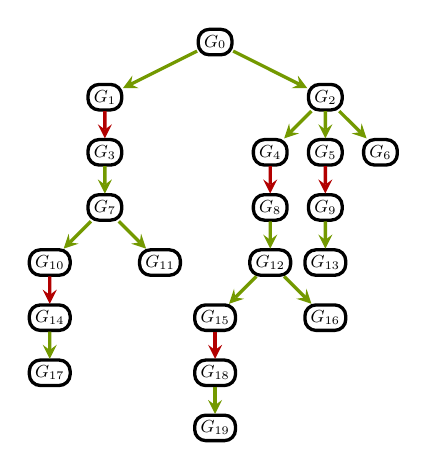
\begin{tikzpicture}[
    scale=0.7,
    transform shape,
    >=stealth,
    node distance=2.2cm and 2.5cm,
    hypernode/.style={draw, rectangle, rounded corners=4pt, very thick, inner sep=3pt, font=\small\bfseries},
    event/.style={draw=none, font=\normalsize},
    rf/.style={->, thick, dashed, green!60!black},
    co/.style={->, thick, dotted, red!80!black},
    graph box/.style={draw, rectangle, rounded corners=4pt, thick, minimum width=1.4cm, minimum height=1cm, inner sep=0.1cm, minimum size=0cm},
    edge label/.style={midway, very thick, fill=white, font=\footnotesize, inner sep=1pt},
    graph box yellow/.style={graph box, dashed},
    graph box blue/.style={graph box},
    every node/.style={transform shape},
    edge-t1/.style={->, very thick, lime!60!black},
    edge-t2/.style={->, very thick, red!70!black},
    circ-label-t1/.style={text=black, inner sep=1pt, font=\normalsize, scale=1.2},
    circ-label-t2/.style={text=black, inner sep=1pt, font=\normalsize, scale=1.2}
]


\node[hypernode] (G0) at (0,0) {$G_0$};

\node[hypernode] (G1) at (-2,-1) {$G_1$};

\node[hypernode] (G2) at (2,-1) {$G_2$};

\node[hypernode] (G3) at (-2,-2) {$G_3$};

\node[hypernode] (G4) at (1,-2) {$G_4$};

\node[hypernode] (G5) at (2,-2) {$G_5$};

\node[hypernode] (G6) at (3,-2) {$G_6$};

\node[hypernode] (G7) at (-2,-3) {$G_7$};

\node[hypernode] (G8) at (1,-3) {$G_8$};

\node[hypernode] (G9) at (2,-3) {$G_9$};

\node[hypernode] (G10) at (-3,-4) {$G_{10}$};

\node[hypernode] (G11) at (-1,-4) {$G_{11}$};

\node[hypernode] (G12) at (1,-4) {$G_{12}$};

\node[hypernode] (G13) at (2,-4) {$G_{13}$};

\node[hypernode] (G14) at (-3,-5) {$G_{14}$};

\node[hypernode] (G15) at (0,-5) {$G_{15}$};

\node[hypernode] (G16) at (2,-5) {$G_{16}$};

\node[hypernode] (G17) at (-3,-6) {$G_{17}$};

\node[hypernode] (G18) at (0,-6) {$G_{18}$};

\node[hypernode] (G19) at (0,-7) {$G_{19}$};


%% Hyper Edges

\draw[edge-t1] (G0) -- (G1);

\draw[edge-t1] (G0) -- (G2);

\draw[edge-t2] (G1) -- (G3);

\draw[edge-t1] (G2) -- (G4);

\draw[edge-t1] (G2) -- (G5);

\draw[edge-t1] (G2) -- (G6);

\draw[edge-t1] (G3) -- (G7);

\draw[edge-t2] (G4) -- (G8);

\draw[edge-t2] (G5) -- (G9);

\draw[edge-t1] (G7) -- (G10);

\draw[edge-t1] (G7) -- (G11);

\draw[edge-t1] (G8) -- (G12);

\draw[edge-t1] (G9) -- (G13);

\draw[edge-t2] (G10) -- (G14);

\draw[edge-t1] (G12) -- (G15);

\draw[edge-t1] (G12) -- (G16);

\draw[edge-t1] (G14) -- (G17);

\draw[edge-t2] (G15) -- (G18);

\draw[edge-t1] (G18) -- (G19);

\end{tikzpicture}
\captionof{figure}{The transition system $\mathcal{D}(\ref{ex:lll})$}
\label{lll-full}
  \end{minipage}
  \hfill
  \begin{minipage}[t]{0.48\textwidth}
    \centering
    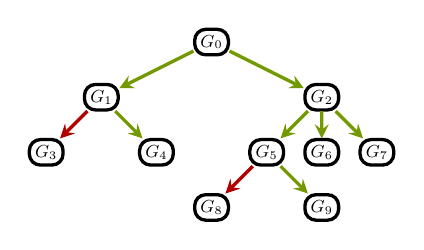
\begin{tikzpicture}[
    scale=0.7,
    transform shape,
    >=stealth,
    node distance=2.2cm and 2.5cm,
    hypernode/.style={draw, rectangle, rounded corners=4pt, very thick, inner sep=3pt, font=\small\bfseries},
    event/.style={draw=none, font=\normalsize},
    rf/.style={->, thick, dashed, green!60!black},
    co/.style={->, thick, dotted, red!80!black},
    graph box/.style={draw, rectangle, rounded corners=4pt, thick, minimum width=1.4cm, minimum height=1cm, inner sep=0.1cm, minimum size=0cm},
    edge label/.style={midway, very thick, fill=white, font=\footnotesize, inner sep=1pt},
    graph box yellow/.style={graph box, dashed},
    graph box blue/.style={graph box},
    every node/.style={transform shape},
    edge-t1/.style={->, very thick, lime!60!black},
    edge-t2/.style={->, very thick, red!70!black},
    circ-label-t1/.style={text=black, inner sep=1pt, font=\normalsize, scale=1.2},
    circ-label-t2/.style={text=black, inner sep=1pt, font=\normalsize, scale=1.2}
]


\node[hypernode] (G0) at (0,0) {$G_0$};

\node[hypernode] (G1) at (-2,-1) {$G_1$};

\node[hypernode] (G2) at (2,-1) {$G_2$};

\node[hypernode] (G3) at (-3,-2) {$G_3$};

\node[hypernode] (G4) at (-1,-2) {$G_4$};

\node[hypernode] (G5) at (1,-2) {$G_5$};

\node[hypernode] (G6) at (2,-2) {$G_6$};

\node[hypernode] (G7) at (3,-2) {$G_7$};

\node[hypernode] (G8) at (0,-3) {$G_8$};

\node[hypernode] (G9) at (2,-3) {$G_9$};



%% Hyper Edges

\draw[edge-t1] (G0) -- (G1);

\draw[edge-t1] (G0) -- (G2);

\draw[edge-t2] (G1) -- (G3);

\draw[edge-t1] (G1) -- (G4);

\draw[edge-t1] (G2) -- (G5);

\draw[edge-t1] (G2) -- (G6);

\draw[edge-t1] (G2) -- (G7);

\draw[edge-t2] (G5) -- (G8);

\draw[edge-t1] (G5) -- (G9);

\end{tikzpicture}
\captionof{figure}{The compressed transition system $\mathcal{D}(\ref{ex:lll})$}
\label{lll-comp}
  \end{minipage}
\begin{example}
Consider the following program.

\begin{equation*}
  \tag{\textsc{L+L+L}}
  \label{ex:lll}
  \inarr{ 
\lockInst{l} \\
\unlockInst{l} \\
}{ 
\lockInst{l} \\
\unlockInst{l} \\
}{
\lockInst{l} \\
\unlockInst{l} \\
}
\end{equation*}

This program consists of three threads, each of which attempts to acquire a lock and subsequently release it. It has $3!$ execution graphs. The complete $\mathcal{D}(\ref{ex:lll})$ tree of this program without tree compression is depicted in \cref{lll-full} and
with compression in \cref{lll-comp}.
With $B=5$, the uncompressed tree requires 20 clones and re-execution but the compressed tree only 10.
%When running \testor with $\mathcal{B} = 4$ over this tree, approximately 20 graph clonings and re-executions must take place per iteration. However, when running \testor with $\mathcal{B} = 5$ over the compressed $\mathcal{D}(\ref{ex:lll})$ tree, as depicted in \cref{lll-comp}, only approximately 10 graph clonings and re-executions are required, reflecting a twofold reduction in overhead.
\qed
\end{example}
\end{tcolorbox}


\begin{comment}
\subsection{OLD TEXT}

\subsection{Estimation with The \trust Algorithm}
Stateless model checking is a verification approach for bounded concurrent programs that systematically explores the program’s execution space without explicitly storing program states. Instead, it repeatedly re-executes the program under different thread scheduling decisions to uncover concurrency bugs such as data races, deadlocks, or assertion violations. To reduce the number of redundant interleavings explored, SMC is typically combined with a dynamic partial order reduction (\dpor) algorithm.

\dpor reduces redundancy by grouping execution traces into equivalence classes that preserve relevant semantic properties. %Common notions of equivalence include execution graph equivalence  (also known as Mazurkiewicz trace equivalence)\cite{maz}, as well as coarser relations such as Reads-From (RF) equivalence \cite{coarser}.
Common notions of equivalence partitioning include Mazurkiewicz trace equivalence \cite{maz} (as well as its generalized version for weak memory models, the Shasha-Snir \cite{shasha} equivalence partitioning), along with coarser relations such as Reads-From (RF) equivalence \cite{coarser}. Each equivalence class can be represented by an execution graph with appropriate relations.

A model checker typically guarantees to explore at least one execution from every equivalence class. It is said to be optimal if it explores exactly one execution per class.
\subsubsection{The \trust Algorithm}

The \trust algorithm is the state-of-the-art stateless model model checking algorithm that achieves optimality while using only polynomial space with respect to the size of the program. 
We briefly outline how \trust operates. %Conceptually, \trust constructs a tree of all consistent execution graphs permitted by the memory model. It starts from the initial graph, which contains only the Init event, and incrementally builds new graphs by adding one event at a time. At each step, \trust selects an enabled thread and invokes an interpreter to execute it until the next memory event is produced.
Conceptually, \trust starts from the initial execution graph and incrementally explores all possible consistent extensions permitted by the memory model. Each constructed graph represents an equivalence class of executions. At each step, the algorithm  schedules one of the enabled threads and recursively explores all possible reorderings of events in a depth-first manner. The exploration terminates once all equivalence classes have been enumerated.

An execution graph initially contains only the \texttt{init} event and is expanded incrementally by adding an event that represents the next operation interpreted from a scheduled enabled thread. When a read event is added, \trust expands the search space by forward visiting different consistent RF relationships relative to existing writes on the same memory location. When a write event is added, \trust expands the search space in two ways: (1) similarly to the case of read events, it forward revisits different consistent MO relationships relative to existing write events, and (2) it also backward revisits earlier reads in restricted execution graphs—constructed by removing all events that have been added after the read and are not in the PORF-prefix of the recently added write—to account for cases where those reads could now consistently read from the new write in an optimal manner. This means the algorithm does not produce any two equivalent restricted execution graphs after processing any backward revisit.
How \trust decides when to perform a revisit is critical to its guarantee of optimality. Blindly revisiting earlier reads for every newly added write can result in redundant exploration of the same execution graph, thereby violating the algorithm’s optimality guarantee. On the other hand, naively remembering all revisits performed so far to avoid repetition requires exponential memory. To address this, \trust relies on a novel condition called the maximal extension condition, which determines precisely when a revisit is necessary—purely based on the current execution graph, rather than the full program state or previously visited configurations. The maximal extension condition ensures that if two execution graphs differ only in the set of events that would later be removed through backward revisits, then the revisit is performed on exactly one of them. This enables \trust to achieve both completeness and optimality while remaining within polynomial space. Notably, the recursion depth of \trust is bounded by $O(k^2)$, where $k$ is the bound on the concurrent program. 
\begin{figure}[t]
\centering
\begin{tikzpicture}[
    >=stealth,
    node distance=1.4cm and 1.8cm,
    event/.style={draw=none, font=\small},
    rf/.style={->, thick, dashed, green!60!black},
    co/.style={->, thick, dotted, red!80!black},
    ->, thick
]

% First row: G1 to G4
\begin{scope}[xshift=0cm, yshift=0cm]
  \node[event] (g1i) {init};
  \node[event, below=0.7cm of g1i] (g1r1) {$R(x)$};
  \draw[->] (g1i) -- node[midway, left] {$t_1$} (g1r1);
  \draw[rf] (g1i) to[bend left=7] (g1r1);
  \node[below=1.2cm of g1i] {(G1)};
\end{scope}

\begin{scope}[xshift=3cm, yshift=0cm]
  \node[event] (g2i) {init};
  \node[event, below=0.7cm of g2i, xshift=-0.9cm] (g2r1) {$R(x)$};
  \node[event, below=0.7cm of g2i] (g2w2) {$W(x)$};
  \draw[->] (g2i) -- node[midway, left] {$t_1$}(g2r1);
  \draw[->] (g2i) -- node[midway, right] {$t_2$}(g2w2);
  \draw[rf] (g2i) to[bend left=7] (g2r1);
  \node[below=1.2cm of g2i] {(G2)};
\end{scope}

\begin{scope}[xshift=6cm, yshift=0cm]
  \node[event] (g3i) {init};
  \node[event, below=0.7cm of g3i, xshift=-1.0cm] (g3r1) {$R(x)$};
  \node[event, below=0.7cm of g3i] (g3w2) {$W(x)$};
  \node[event, below=0.7cm of g3i, xshift=1.0cm] (g3w3) {$W(x)$};
  \draw[->] (g3i) -- node[midway, left] {$t_1$}(g3r1);
  \draw[->] (g3i) -- node[midway, right] {$t_2$}(g3w2);
  \draw[->] (g3i) -- node[midway, right, xshift=0.3cm] {$t_3$}(g3w3);
  \draw[rf] (g3i) to[bend left=10] (g3r1);
  \draw[co] (g3w2) -- (g3w3);
  \node[below=1.2cm of g3i] {(G3)};
\end{scope}

\begin{scope}[xshift=9cm, yshift=0cm]
  \node[event] (g4i) {init};
  \node[event, below=0.7cm of g4i, xshift=-1.0cm] (g4r1) {$R(x)$};
  \node[event, below=0.7cm of g4i] (g4w2) {$W(x)$};
  \node[event, below=0.7cm of g4i, xshift=1.0cm] (g4w3) {$W(x)$};
  \draw[->] (g4i) -- node[midway, left] {$t_1$}(g4r1);
  \draw[->] (g4i) -- node[midway, right] {$t_2$}(g4w2);
  \draw[->] (g4i) -- node[midway, right, xshift=0.3cm] {$t_3$}(g4w3);
  \draw[rf] (g4i) to[bend left=10] (g4r1);
  \draw[co] (g4w3) -- (g4w2);
  \node[below=1.2cm of g4i] {(G4)};
\end{scope}



% Second row: G5 to G8
\begin{scope}[xshift=0cm, yshift=-2.5cm]
  \node[event] (g5i) {init};
  \node[event, below=0.7cm of g5i, xshift=-1.0cm] (g5r1) {$R(x)$};
  \node[event, below=0.7cm of g5i, xshift=1.0cm] (g5w3) {$W(x)$};
  \draw[->] (g5i) -- node[midway, left] {$t_1$}(g5r1);
  \draw[->] (g5i) -- node[midway, right, xshift=0.3cm] {$t_3$}(g5w3);
  \draw[rf] (g5w3) to[bend left=10] (g5r1);
  \node[below=1.2cm of g5i] {(G5)};
\end{scope}

\begin{scope}[xshift=3cm, yshift=-2.5cm]
  \node[event] (g6i) {init};
  \node[event, below=0.7cm of g6i, xshift=-1.0cm] (g6r1) {$R(x)$};
  \node[event, below=0.7cm of g6i] (g6w2) {$W(x)$};
  \node[event, below=0.7cm of g6i, xshift=1.0cm] (g6w3) {$W(x)$};
  \draw[->] (g6i) -- node[midway, left] {$t_1$}(g6r1);
  \draw[->] (g6i) -- node[midway, right] {$t_2$}(g6w2);
  \draw[->] (g6i) -- node[midway, right, xshift=0.3cm] {$t_3$}(g6w3);
  \draw[rf] (g6w3) to[bend left=10] (g6r1);
  \draw[co] (g6w2) -- (g6w3);
  \node[below=1.2cm of g6i] {(G6)};
\end{scope}

\begin{scope}[xshift=6cm, yshift=-2.5cm]
  \node[event] (g7i) {init};
  \node[event, below=0.7cm of g7i, xshift=-1.0cm] (g7r1) {$R(x)$};
  \node[event, below=0.7cm of g7i] (g7w2) {$W(x)$};
  \node[event, below=0.7cm of g7i, xshift=1.0cm] (g7w3) {$W(x)$};
  \draw[->] (g7i) -- node[midway, left] {$t_1$}(g7r1);
  \draw[->] (g7i) -- node[midway, right] {$t_2$}(g7w2);
  \draw[->] (g7i) -- node[midway, right, xshift=0.3cm] {$t_3$}(g7w3);
  \draw[rf] (g7w3) to[bend left=10] (g7r1);
  \draw[co] (g7w3) -- (g7w2);
  \node[below=1.2cm of g7i] {(G7)};
\end{scope}

\begin{scope}[xshift=9cm, yshift=-2.5cm]
  \node[event] (g8i) {init};
  \node[event, below=0.7cm of g8i, xshift=-1.0cm] (g8r1) {$R(x)$};
  \node[event, below=0.7cm of g8i] (g8w2) {$W(x)$};
  \draw[->] (g8i) -- node[midway, left] {$t_1$}(g8r1);
  \draw[->] (g8i) -- node[midway, right] {$t_2$}(g8w2);
  \draw[rf] (g8w2) to[bend left=10] (g8r1);
  \node[below=1.2cm of g8i] {(G8)};
\end{scope}

% Second row: G9 to G10
\begin{scope}[xshift=0cm, yshift=-5cm]
  \node[event] (g9i) {init};
  \node[event, below=0.7cm of g9i, xshift=-1.0cm] (g9r1) {$R(x)$};
  \node[event, below=0.7cm of g9i] (g9w2) {$W(x)$};
  \node[event, below=0.7cm of g9i, xshift=1.0cm] (g9w3) {$W(x)$};
  \draw[->] (g9i) -- node[midway, left] {$t_1$}(g9r1);
  \draw[->] (g9i) -- node[midway, right] {$t_2$}(g9w2);
  \draw[->] (g9i) -- node[midway, right, xshift=0.3cm] {$t_3$}(g9w3);
  \draw[rf] (g9w2) to[bend left=10] (g9r1);
  \draw[co] (g9w2) -- (g9w3);
  \node[below=1.2cm of g9i] {(G9)};
\end{scope}

\begin{scope}[xshift=3cm, yshift=-5cm]
  \node[event] (g10i) {init};
  \node[event, below=0.7cm of g10i, xshift=-1.0cm] (g10r1) {$R(x)$};
  \node[event, below=0.7cm of g10i] (g10w2) {$W(x)$};
  \node[event, below=0.7cm of g10i, xshift=1.0cm] (g10w3) {$W(x)$};
  \draw[->] (g10i) -- node[midway, left] {$t_1$}(g10r1);
  \draw[->] (g10i) -- node[midway, right] {$t_2$}(g10w2);
  \draw[->] (g10i) -- node[midway, right, xshift=0.3cm] {$t_3$}(g10w3);
  \draw[rf] (g10w2) to[bend left=10] (g10r1);
  \draw[co] (g10w3) -- (g10w2);
  \node[below=1.2cm of g10i] {(G10)};
\end{scope}

\end{tikzpicture}
\caption{Execution graphs illustrating different read-from and coherence orders among three threads.}
\label{exec-graphs}
\end{figure}


\begin{figure}[h]
\centering
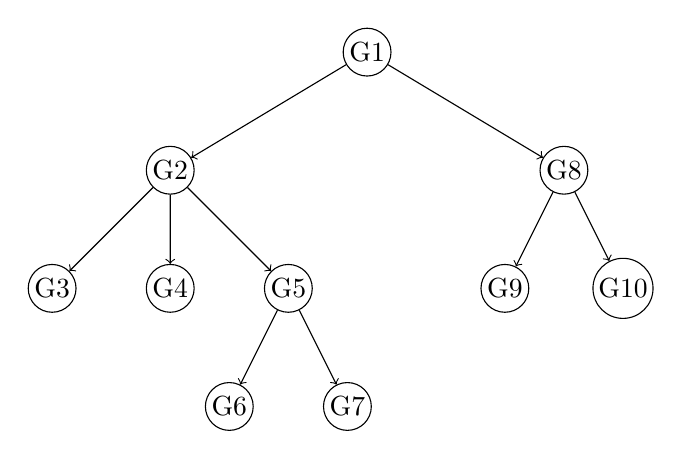
\begin{tikzpicture}[
  level distance=1.5cm,
  sibling distance=1.5cm,
  edge from parent/.style={->, draw},
  every node/.style={circle, draw, minimum size=6mm, inner sep=1pt},
  level 1/.style={sibling distance=5cm},
  level 2/.style={sibling distance=1.5cm}
  ]

\node (G1) {G1}
  child {node (G2) {G2}
    child {node (G3) {G3}}
    child {node (G4) {G4}}
    child {node (G5) {G5}
        child {node (G6) {G6}}
        child {node (G7) {G7}}
        }
  }
  child {node (G8) {G8}
    child {node (G9) {G9}}
    child {node (G10) {G10}}
  };

\end{tikzpicture}
\caption{backtracking tree tree of Trust over execution graphs.}
\label{fig:graph-tree}
\end{figure}

\begin{example}
\label{example1}
   Consider a simple concurrent program with three threads: $t_1$, $t_2$, and $t_3$, where $t_1$ reads from a shared variable $x$, and both $t_2$ and $t_3$ write to $x$. Suppose we fix a schedule where $t_1$ executes first, followed by $t_2$ and then $t_3$. \trust begins by exploring the execution graph in which the read from $t_1$ observes the initial value of $x$ (denoted $\mathsf{init}$), corresponding to graph G1 in Figure~\ref{exec-graphs}.Next, when the write from $t_2$ is scheduled, \trust first considers the case where the write is ordered after the read via a from-read ($\mathsf{fr}$) edge, yielding graph G2. It then explores a backward revisit that allows the read to instead read from this write, resulting in graph G7.From G2, \trust proceeds to schedule the write from $t_3$ and explores two possible modification orders: one where the write from $t_3$ follows the write from $t_2$ (G3), and one where it precedes it (G4). It then explores additional graphs where the read reads from the newly scheduled write (G5 and G6), depending on the modification order and visibility of writes. From G7, \trust explores the two possible modification orders introduced by scheduling the write from $t_3$, resulting in graphs G8 and G9.It is important to notice that from G7 \trust does not explore the possibility when the read can read from the write from $t_3$. This is because G7 does not satisfy the maximal extension condition.  
\qed
\end{example}

%\subsubsection{Estimation with the backtracking Tree of \trust}
%The \trust algorithm can be viewed as implicitly exploring a tree whose leaves represent all complete execution graphs. Because \trust is optimal, each recursive call generates a unique feasible execution, establishing a one-to-one correspondence between leaves of the tree and execution graphs of the input program. Each node in this tree corresponds to a recursive call in the algorithm, and its structure mirrors the recursive control flow.\footnote{The \trust algorithm may also explore some infeasible execution graphs, but the corresponding recursive calls can be easily identified in polynomial time and excluded from both the model and the estimation procedure.}
%
%At each node, branching is determined solely by the current recursive call, making the tree amenable to Knuth’s method for estimating its size via random sampling. To apply Knuth’s algorithm, we modify \trust to randomly select one consistent RF/MO relation at each recursive step rather than exploring all possibilities. This yields an unbiased estimator for Problem~\ref{prob1}.
%
%Equivalently, an alternative way of interpreting the idea is that we can define a nondeterministic polynomial time Turing machine that simulates the \trust algorithm and, whenever multiple recursive subcalls are spawned, nondeterministically proceeds with exactly one of them. Notably, this machine is a generator, since every run accepts. As discussed at the start of this section, applying Knuth’s method to this Turing machine yields an unbiased estimator of the true count. 
%


%\subsection{Estimation with a DAG Structure}
%While \trust organizes execution graphs into a tree structure in an elegant and principled way, it is designed for a one-pass exhaustive traversal rather than for estimation. Nonetheless, the resulting tree can be quite balanced: the shortest paths are clearly linear in the program bound, whereas the longest paths may be quadratic due to repeated backward revisits. On the other hand, the concurrent system $M_{p}^{SC}$  as defined in the preliminaries, possibly offers a more natural model for this purpose. Recall that the states of $M_{p}^{SC}$ are pairs of controls(program counters) and execution graphs where no two states share the same execution graph. The transitions between states capture valid thread scheduling choices, in contrast to the estimator defined by \trust, where the execution graphs are related by partial order based semantic. 
%
%The graph induced by $M_{p}^{SC}$ naturally forms a layered DAG, where each path corresponds to a feasible execution under some thread interleaving, and all executions that yield the same execution graph converge to the same final state. 
%
%\begin{example}
%Consider a simple concurrent program $P$ with two threads, each executing a single event: thread $t_1$ performs a write to \texttt{x}, and thread $t_2$ performs a read %from \texttt{x}. As illustrated in Figure~\ref{egraphs}, the program admits five execution graphs, among which (3) and (4) are complete execution graphs. %Figure~\ref{structures} provides two structural views of the behavior space: the left diagram depicts the backtracking tree implicitly constructed by the \trust algorithm %under the scheduling order $t_1 \rightarrow t_2$, while the right diagram shows the corresponding concurrent system $M_{P}^{SC}$.
%\qed
%\end{example}
%
%\input{graph-example}
\end{comment}



\subsection{Related Work: The GenMC Estimator}

The state estimation problem was also considered in \cite{gator}, where the authors give a randomized procedure based on the \trust algorithm.
However, as we show below, that estimator is not an unbiased estimator; thus, even with exponentially many samples,
it has no guarantees to converge to the correct answer.
Experimentally, the estimator converges to incorrect values quite frequently.

%\citet{gator} describe a biased probabilistic estimator for \trust. 
%
% However, the proposed estimator was biased.
%% likely because the authors did not recognize that the backtracking tree implicitly generated by the \trust algorithm already provides a natural structure for unbiased estimation.

%The method follows Knuth-style single-path sampling. 
The procedure is also based on the \trust algorithm, and proceeds as follows.
First, it preferentially schedules writes over reads.
For each read or write event, it explores one of the forward-revisits uniformly at random. 
Instead of computing the estimate on the fly, it records the number of values each read can read from. 
In case a new write is added and \trust detects that a backward revisit would be required, the estimator
does not perform the backward revisit but increments the map entry for any read that could read from this new value by one. 
At the end, it takes the product of the ``possible reads-from'' counts for every read and the ``possible modification order" 
for every write to produce the final estimate.

Intuitively, the estimator assumes one can generate all graphs in $\mathcal{T}(P)$ 
without any backward revisits, simply by scheduling write events before read events.
%% (when only read events are enabled, the scheduler proceed with threads uniformly at random). 
When this assumption holds, the estimate is unbiased. 
However, the assumption may not hold. 
Since the algorithm forbids backward revisits, it may omit graphs 
reachable only via backward revisits and produce a biased estimate.
%% The estimator can be very biased. The experiment from \citet{gator}  also showed that the algorithm is biased and can converge to wrong values quite frequently.
\begin{tcolorbox}[
    colback=SkyBlue!5,
    colframe=blue!20,
    boxrule=1pt,
    arc=2pt,
    width=\textwidth,
    boxsep=5pt,
    left=5pt,
    right=5pt,
    top=5pt,
    bottom=5pt
]

\noindent
\begin{minipage}[t]{0.7\textwidth}
\begin{example}
Consider the following program. It has 4 execution graphs: 
one where the line $a_2:=x$ reads from the $\init$, one where it reads from $x:=1$, and two where it reads from $x:=2$. 
The algorithm in \cite{gator} runs as follows. 
It first schedules $t_1$ and writes 1 to $x$. 
Then since both threads are enabled with a read, the scheduler picks one uniformly at random.
A case analysis of the two possibilities shows that the expected value of the estimator is
3.5.
\end{example}
\end{minipage}%
\hfill
\begin{minipage}[t]{0.3\textwidth}
\vspace{0pt}
\begin{equation*}
  \tag{\textsc{wrww+rr}}
  \label{ex:wrww+rr}
  \inarr{ 
\writeInst{x}{1} \\
\readInst{a_1}{x} \\
\writeInst{x}{2} \\
\writeInst{y}{1} 
}{ 
\readInst{a_2}{x} \\
\text{if } a_2 = 2 \\
\readInst{a_2}{y }}
\end{equation*}
\end{minipage}%

\begin{comment}
\vspace{0.3cm}

Case A: the scheduler proceeds with $t_1$. Since the remaining events of $t_1$ are writes, the scheduler will continue proceeding with $t_1$ until it finishes. Up to this point, the estimation is $1$ because no forward revisit is needed. It then schedules the first event of $t_2$. There are three possible read-from values (including the initial value), so the estimator will store the knowledge that the read $a_2:=x$ has three possible forward revisits. With probability $2/3$, the estimator explores the case that $a_2$ does not read $2$, then $t_2$ terminates and the estimator returns 3. With probability $1/3$, $a_2$ reads  $2$ and enters the if-branch and reads $y$, which has two possible values, so the estimator returns $6$.

Case B: the scheduler proceeds with $t_2$. At that moment, the read has two possible forward revisits (from $\init$ and from the write $x:=1$), so the estimator records $2$ for this read. Regardless of which value $a_2$ reads in this case, it does not enter the if-branch and terminates. $t_1$ is then scheduled, and the estimator detects a backward revisit and updates that the earlier read into $a_2$ actually had three possible values to read from; however, because the algorithm forbids backward revisits, it does not explore that alternative and still returns $3$.

Thus the expected output in Case A is $(2/3)\times3 + (1/3)\times6 = 4$, and in Case B it is $3$. 
Thus, the expected value of the estimator is $0.5\times 4 + 0.5\times 3 = 3.5$.
\end{comment}
\qed
\end{tcolorbox}
